\documentclass{fiwthesis}

% ========
%  Pakete
% ========

\usepackage{textgreek}           % griechische Buchstaben außerhalb des Math-Mode
\usepackage{amsmath}             % zentrierte Formeln
\usepackage{amssymb}             % erweiterter Formelsatz mathem. Symbole

\usepackage{boldline}            % breitere Linien in Tabellen
\usepackage{booktabs}            % typographisch richtige Tabellen setzen
\usepackage{tabularx}            % Erweiterte Tabellendarstellung
\usepackage{multirow}            % Spalte über mehrere Zeilen oder Spalten ausdehnen
\usepackage{xltabular}           % Zeilenumbrüche in tabularx erlauben

\usepackage{graphicx}            % ermöglicht das Einbinden von Grafiken
\usepackage{subcaption}          % mehrere Bilder in einem Bild
\usepackage{pgfplots}            % Grafiken erzeugen
\usepackage{smartdiagram}        % schnelle und einfache Grafiken

\newtheorem{definition}{Definition}

% Commands for TODOs
% \usepackage[pdftex,dvipsnames]{xcolor}  % Coloured text etc.

\usepackage{xargs}
\setlength{\marginparwidth }{2cm}
\usepackage[colorinlistoftodos,prependcaption,textsize=tiny]{todonotes}
\newcommandx{\unsure}[2][1=]{\todo[linecolor=red,backgroundcolor=red!25,bordercolor=red,#1]{#2}}
\newcommandx{\change}[2][1=]{\todo[linecolor=blue,backgroundcolor=blue!25,bordercolor=blue,#1]{#2}}
\newcommandx{\info}[2][1=]{\todo[linecolor=OliveGreen,backgroundcolor=OliveGreen!25,bordercolor=OliveGreen,#1]{#2}}
\newcommandx{\improvement}[2][1=]{\todo[linecolor=Plum,backgroundcolor=Plum!25,bordercolor=Plum,#1]{#2}}
\newcommandx{\thiswillnotshow}[2][1=]{\todo[disable,#1]{#2}}

% ===========
%  Metadaten
% ===========

\thesis{Master-Thesis}
\title{Homomorphic Post-Quantum Cryptography - Evaluation of Module Learning with Error in Homomorphic Cryptography}
\author{Pascal Stehling}
\matrnr{455051}
\bdate{18.12.1997}
\bcity{Wismar}
\supervisor{Prof.~Dr.-Ing.~habil.~Andreas Ahrens}
% \secsupervisor{ZWEITBETREUER}
\keywords{Logik, Mathematik}

% Metadaten in die PDF-Datei schreiben
\makepdfmetadata

% ===============
%  Präambel
% ===============

% PGF Kompatibilitätseinstellung
\pgfplotsset{width=0.95\textwidth,compat=newest}

% % Bibliographie einbinden
\bibliography{quellen}

% Glossar einbinden
% this cant be removed, for some reason the build breaks
\newdualentry{dos}% label
{DoS}% short form
{Denial of Service}% long form
{Ein Denial of Service (im Deutschen: Dienstverweigerung) ist ein Angriffe auf Computer- oder Netzwerksysteme, wobei das Zielsystem durch Überlastung oder durch andere Mittel außer Betrieb gesetzt wird}% description


% Abkürzungen einbinden
%\gls{}         normal zu nutzen (erstes Mal: 'lange Form (kurze Form)'), danach nur 'kurze Form'
%\glspl{}       wie \gls{} nur als Plural
%\acrfull{qrc}  gibt volle Form ('lange Form (kurze Form)') egal wo
%\acrlong{qrc}  gibt lange Form ('lange Form') egal wo
%
%\newacronym{tag}{short}{long}
\newacronym{lamp}{LAMP}{Linux, Apache, MySQL, PHP}
\newacronym{qrc}{QR-Code}{Quick Response Code}


% Symbole einbinden
\newglossaryentry{symb:phi}{
  name=$\phi$,
  description={Ein beliebiger Winkel},
  sort=symbolphi, type=symbolslist
}

\newglossaryentry{symb:e}{
  name=$e$,
  description={Die Eulersche Zahl},
  sort=symbole, type=symbolslist
}


% % Glossar- und Abkürzungsverzeichniserstellung
% \makeglossaries{}

% Index erzeugen
\makeindex[
  intoc=true,
  title=Index,
  columns=2]{}
\indexsetup{headers={\indexname}{\indexname}}

% ===============
%  Eigene Makros
% ===============

\newcommand*{\code}[1]{\texttt{#1}}

\begin{document}

% Titelseite
\maketitle

\maketask{
In 2009, Craig Gentry published the first fully homomorphic encryption (FHE) algorithm in his PhD dissertation. With that it was possible for the first time to do any number of calculations on encrypted messages without having to decrypt them. Since the discovery of this first FHE algorithm, other such algorithms have been developed, but instead of using Ideal Lattices as the mathematical foundation, newer ones tend to use the Learning with Errors (LWE) and Ring-LWE (RLWE) problems.

In July 2022, the American National Institute of Standards and Technology (NIST) published the first group of winners of its competition for quantum-safe algorithms. The winner for general asymmetric encryption was the CRYSTALS-Kyber algorithm, which is based on Module-LWE (MLWE). This is an extension of the RLWE method in which polynomials in higher dimensions (vectors and matrices) are used. Even though it needs more computational power, in contrast to RLWE, it can be offset through parallelization of the calculations and higher security.

With these two distinct developments, the questions can be asked, if it possible to combine them and see if it’s possible to transfer existing FHE cryptosystems, which are based on RLWE to the MLWE method. This will first be researched theoretically and then verified with practical tests. 
These tests will be used to examine the advantages and disadvantages of the different Methods in terms of various properties, such as computation speed, error rate during decryption, number of possible calculations without errors and others. In order to structure these tests and thus establish good comparability, a test concept will be created in this thesis. 
At the end, the following question should be answered: Are their practical advantages to transferring existing FHE systems from RLWE to MLWE or whether the associated increased computing effort nullifies the advantages again?}

\makeabstract{
  Abstract.
}

\maketoc[compact]

% ==========
%  Textteil
% ==========

\chapter{Introduction}
\label{Introduction}

% \section{Background}

In the early months of 1978, one of the most significant cryptographic systems, the RSA system \cite{RSA}, was published. With the advent of the Internet in the 1990s and the subsequent need for secure data transfer, it became one of the most widely used encryption schemes to date. In the subsequent period of slightly more than half a year, two of the authors of the RSA paper published a new concept, based on the RSA concept, which they designated ''privacy homomorphism`` \cite{Rivest1978}. This concept would later be known as homomorphic encryption. This is an encryption system whereby operations can be executed directly on encrypted data, eliminating the necessity of first decrypting it, running the operations, and then encrypting it again. Such a system would not only eliminate the necessity for decryption and encryption at the processing stage, it would also ensure that the plain text is not accessible to the party undertaking this processing. However, at the system's inception, only one operation was feasible: multiplication. To develop a system capable of general computing, the addition operation was necessary as a second operation, as these two operations enable the recreation of all other operations at the bit level. Unfortunately, the creation of a homomorphic encryption scheme with unlimited additions and multiplications, also known as full homomorphic encryption (FHE), proved to be a formidable challenge.\\
In 1994, Peter Shor published his algorithm \cite{Shor}, which describes how a quantum computer could factorize numbers in polynomial time. In contrast to classical computers, for which this problem is categorized as a hard problem. As the RSA cryptosystem is based on this exact issue being hard to solve, it would be possible to find the private key for any public key, thus undermining the cryptosystem's security. Fortunately, no quantum computer capable of such an operation was anywhere near availability at the time, so this problem remained theoretical.\\
Approximately a decade later, in 2005, O. Regev devised a novel mathematical framework, termed Learning with Error (LWE) \cite{Regev2005OnLL}, which enables the construction of new cryptosystems. This framework is based on an error term within a linear system of equations constructed on a lattice. The mathematical problem that he exploits for security is the hardness of the shortest vector problem (SVP). There are variants of this problem, called Ring-LWE, where a polynomial is used instead of a matrix, and M-LWE, which mixes Ring-LWE and the (Plain-)LWE together, resulting in matrices of polynomials. In 2009, Craig Gentry published the first full-homomorphic encryption scheme \cite{Gentry2009AFH}. This development prompted renewed optimism regarding the advancement of FHE schemes, as it became evident that the concept was indeed feasible. However, the primary challenge that remained was the issue of performance. To enhance the efficiency of this scheme, the initial version, which was based on the ideal lattice, was adapted to the R-LWE scheme. Over time, significant advancements have been made in the development of these FHE schemes, which are constructed on basis of R-LWE \cite{FHESurvey}. However, the primary challenge persists, namely the performance, which is frequently 1000s of times slower than operations on the plain text.\\
In recent years, there has been a resurgence of interest in quantum computers as various companies compete to develop the first practical and useful quantum computer \cite{googleQuantumComputing} \cite{ibmQuantumComputing}. Consequently, the performance of these computers has been steadily improving. If the promises made are accurate, it is possible that in 10 years, viable quantum computers will be available on the market. These computers could run Shor's Algorithm and thereby breach the security of RSA (and other) cryptosystems, potentially undermining the security of the internet as it currently stands. To circumvent such potential issues, the US National Institute of Standards and Technology (NIST) initiated an open competition in 2016, wherein individuals could submit novel cryptographic systems for analysis. Research teams from around the globe would then endeavor to identify vulnerabilities in these systems. In 2022, the NIST announced the first four winners \cite{nistAnouncement}, three of which were based on LWE. The two most recommended systems, CRYSTALS-Kyber \cite{CyrstalsKyber} and CRYSTALS-Dilithium \cite{crystalsDilithium}, are both based on M-LWE.


% \section{Goal of this Thesis}

In light of these recent advancements in M-LWE-based encryption schemes and the established R-LWE-based homomorphic encryption schemes, a question arises concerning the potential for integrating these two approaches: Is it possible to port the R-LWE-based homomorphic encryption schemes to M-LWE, and whether this results in an improvement in performance? Should the advantages outweigh the disadvantages, this would facilitate new synergies between the current endeavour to enhance the security of a post-quantum internet and the construction of efficient and dependable homomorphic encryption algorithms. For instance, enhanced and high-performing implementations or even hardware accelerators could be reused, thereby enhancing the efficacy of homomorphic encryption while simultaneously reducing the cost of development.

The thesis is divided into five principal sections. The first section of the thesis provides an introduction to the mathematical background, wherein all necessary mathematical operations will be explained in sufficient detail. Subsequently, the LWE problems will be described in greater detail, and a basic LWE-based encryption scheme will be constructed. The scheme is capable of functioning on Plain-, Ring-, and Module-LWE. Following this, homomorphic encryption will be outlined, and the LWE-based encryption scheme will be expanded to become homomorphic for all three LWE modes. These schemes will then be evaluated based on their memory usage, processing performance, and calculation depth. Ultimately, the aforementioned question will be addressed based on these findings.

\chapter{Mathematical Background}
\label{MathBack}

In order to understand the mathematical concepts behind the encryption algorithms described here, some basic concepts are explained here. However, you should have a basic knowledge of linear algebra and polynomial calculus.

\section{Lattice}

\section{Shortest Vector \& Closest Vector Problem}

\section{Polynomial Rings}
- explain also the modulus


\chapter{Learning with Errors}
\label{LWE}

In this section, we will take a closer look at the Learning with Errors (LWE) algorithm (also called Plain LWE) and its different versions, namely Ring LWE (R-LWE) and Module LWE (M-LWE).

\section{The Learning with Errors Problem}

In 2005, Regev first described the LWE problem \cite{Regev2005OnLL}. He also proved its hardness, but we won't go into those details here. The basic idea is to add an error vector to a linear system of equations. This makes the normally trivially solvable system surprisingly hard to solve.

In more mathematical terms, $\mathbb{Z}_q = \mathbb{Z}/n$, $A \in \mathbb{Z}_q^{n \times m}$, $s \in \mathbb{Z}_q^m$, $b \in \mathbb{Z}_q^n$, with which we can form the linear system of equations, where $A$ and $b$ are given and the vector $s$ represents the unknowns we want to retrieve

$$\textbf{A}\cdot \textbf{s} = \textbf{b}$$

Or written as system of equations it would look like:
$$
  \setlength\arraycolsep{0pt}
  \begin{array}{ c  >{{}}c<{{}} c  >{{}}c<{{}}  c >{{}}c<{{}}  c @{{}={}} c }
    A_{11}s_1 & + & A_{12}s_2 & + & \cdots & + & A_{1m}s_m & b_1    \\
    A_{21}s_1 & + & A_{22}s_2 & + & \cdots & + & A_{2m}s_m & b_1    \\
    \vdots    &   & \vdots    &   & \vdots &   & \vdots    & \vdots \\
    A_{n1}s_1 & + & A_{n2}s_2 & + & \cdots & + & A_{nm}s_m & b_n    \\
  \end{array}
$$

This can easily be solved with the Gaussian algorithm. But if we just add an error vector $e \in \mathbb{Z}_q^n$ with small values, it becomes surprisingly hard. The hardness is based on variants of the Shortest Vector Problem (SVP), which describes the hardness of finding the shortest vector in the lattice. This is easily solvable in smaller dimensions, but gets harder as the dimensions are increased. The equation after adding the small error term is the following:

$$\textbf{A}\cdot \textbf{s} + \textbf{e}= \textbf{b}$$

This is the main equation that all LWE problems are based on. Most of the differences will come from the ring or the dimensions used.

\info[inline]{Maybe going more into detail of the SVP or general the hardness of the LWE Problem?}

\section{LWE based encryption scheme}
\label{sec:Lwe-Encryption}

In this section, we will describe a simple LWE-based encryption scheme and how it can be converted to R-LWE and M-LWE. The following algorithm is loosely based on the Kyber \cite{CyrstalsKyber} scheme, with some simplifications.

All calculations are done in the ring $R = \mathbb{Z}_q$, where $q$ is the modulus. If values from $R$ are chosen uniformly, this is denoted by $x \leftarrow R$. Otherwise, if small values are chosen from $R$, this is written as $x \leftarrow \chi_R$. This can be done by choosing uniformly from a set of small numbers all in $R$ (e.g., ${-4,\ldots, 4}$ if $q$ is big enougth), or by choosing from an error distribution, such as the discrete Gaussian, as described in \cite{Regev2005OnLL}.

The following three algorithms describe the example schema. Algorithm \ref{alg: SampleLweKeyGen}, the key generation, describes how to generate the private key $pk$ and the secret key $sk$. It uses the LWE problem as described above. The secret key, which the owner should never share, is the vector $s$. The public key $pk$, which can be shared, consists of the transformation matrix $A$ and the transformed secret key plus the error $b$. The error $e$ is discarded after the computation of $b$. The values of $e$ and $s$ should be rather small, and $A$ is uniformly sampled from $R$.

\begin{algorithm}[htb]
  \begin{algorithmic}[1]
    \STATE $s \leftarrow \chi_R^n$
    \STATE $A \leftarrow R^{n \times n}$
    \STATE $e \leftarrow \chi_R^n$
    \STATE $b = A\cdot s+e$
    \RETURN $(pk:=(A, b), sk:=s )$
  \end{algorithmic}
  \caption{Sample LWE: KeyGen}
  \label{alg: SampleLweKeyGen}
\end{algorithm}

Algorithm \ref{alg: SampleLweEncryption}, the encryption, describes how to encrypt a message $m$ with the public key $pk$. The errors $e_1$ and $e_2$ are randomly sampled with small values and used to create more uncertainty around the message. The same message can therefore be decrypted with different errors and yield different values. This makes it harder for attackers to find patterns in the decryption. The idea behind $r$ is to select a subset of $A$ and $b$, since $~50\%$ of the values in $r$ will be $0$, meaning that these columns in $A$ and $b$ are irrelevant (multiplied by $0$). This helps to create more entropy between different encryptions, as a different subset of $A$ and $b$ will be used to encrypt each time.

The new values and the public key are used to calculate two values: $u$ and $v$. The first term, $u$, can be considered the cancel term for $b$, where the secret $s$ is missing. $v$ is the actual value term, which is composed of a subset of $b$ with some small error added and the scaled message $m'$. For the scaled message $m' = m*\left\lfloor q/2\right\rfloor$, the message is multiplied with the rounded down version of half the modulus. This operation results in the values of the message $0$ and $1$ in the ring being approximately as distant from each other as possible.

\begin{algorithm}[htb]
  \begin{algorithmic}[1]
    \REQUIRE $m \in \mathbb{Z}_2 = \{0, 1\}$, $pk = (A, b)$
    \STATE $r \leftarrow \{0, 1\}^n$
    \STATE $e_1 \leftarrow \chi_R^n$
    \STATE $u = A^T \cdot r + e_1$
    \STATE $e_2 \leftarrow \chi_R$
    \STATE $v = b^T \cdot r + e_2 + (m*\left\lfloor q/2\right\rfloor)$
    \RETURN $ct := (u, v)$
  \end{algorithmic}
  \caption{Sample LWE: Encryption}
  \label{alg: SampleLweEncryption}
\end{algorithm}

Algorithm \ref{alg: SampleLweDecryption}, the Decryption, describes how to decrypt an ciphertext $ct$ using the secret key $sk$.



\begin{algorithm}[htb]
  \begin{algorithmic}[1]
    \REQUIRE $ct = (u, v)$, $sk = s$
    \RETURN $\left\lfloor \frac{1}{\left\lfloor q/2\right\rfloor}*\left[v-s^T \cdot u\right]_q\right\rceil _2$
  \end{algorithmic}
  \caption{Sample LWE: Decryption}
  \label{alg: SampleLweDecryption}
\end{algorithm}


To get a better understanding, consider the following simplification of the term in algorithm \ref{alg: SampleLweDecryption}.

\begin{align*}
   & \left\lfloor \frac{1}{\left\lfloor q/2\right\rfloor}*\left[v-s^T \cdot u\right]_q\right\rceil _2                                                                                     \\
   & = \left\lfloor \frac{1}{\left\lfloor q/2\right\rfloor}*\left[b^T \cdot r + e_2 + (m*\left\lfloor q/2\right\rfloor)-s^T \cdot (A^T \cdot r + e_1)\right]_q \right\rceil _2             \\
   & = \left\lfloor \frac{1}{\left\lfloor q/2\right\rfloor}*\left[(As+e)^T \cdot r + e_2 + (m*\left\lfloor q/2\right\rfloor)-s^T A^T \cdot r - s^T e_1\right]_q \right\rceil _2            \\
   & = \left\lfloor \frac{1}{\left\lfloor q/2\right\rfloor}*\left[(As)^T \cdot r + e^Tr+ e_2 + (m*\left\lfloor q/2\right\rfloor)-(As)^T \cdot r - s^T e_1\right]_q\right\rceil _2         \\
   & = \left\lfloor \frac{1}{\left\lfloor q/2\right\rfloor}*\left[e^Tr+ e_2 + (m*\left\lfloor q/2\right\rfloor)- s^T e_1\right]_q\right\rceil _2                                          \\
   & = \left\lfloor \frac{e^Tr}{\left\lfloor q/2\right\rfloor}+ \frac{e_2 }{\left\lfloor q/2\right\rfloor}+ m - \frac{s^T e_1}{\left\lfloor q/2\right\rfloor}\right\rceil _2 \\
   & = \left\lfloor m' \right\rceil _2                                                                                                                                       \\
   & = m \in \{0,1\}
\end{align*}
As demonstrated by the calculation, by multiplying the cancellation term $u$ with the secret $s$, the transformation $(As)^T \cdot r$ in $v$ can be canceled out. This results in the message with some error values being added to it. The erroneous message will then be rounded, which will result in the original message. This process will only be successful if all error terms together are smaller than $\frac{q}{4}$. This is due to the fact that the possible values in the message are separated by a distance of $\frac{q}{2}$ from each other. Consequently, all values between $-\frac{q}{4}\mod q=\frac{3q}{4}$ and $\frac{q}{4}$ are rounded back to $0$, while all values between $\frac{q}{4}$ and $\frac{3q}{4}$ are rounded to $1$. Consequently, provided that the message (either $0$ or $\frac{q}{2}$) is not shifted by more than $\frac{q}{4}$, it will remain within the rounding area of the original message.

\info[inline]{Maybe add an image which shows the rounding with an clock}

The current definition of this algorithm allows only $1$ bit to be encoded at the time. This could be improved with some tricks, but for simplicity reasons we wont do that here. 

To observe the functioning of this algorithm in practice, please refer to the example calculation in the appendix, which can be found in Appendix \ref{app:PlainLweCalc}.

\section{Transforming LWE to R-LWE and M-LWE}

To transform the algorithms described above into Ring-LWE, only a few changes need to be made. Most importantly, a polynomial ring will be defined as $R = \mathbb{Z}[x]_q/(x^d+1)$, with the dimension $n=1$, which means that there are only polynomials. Instead of having a vector $r$, it will now be a polynomial in the ring $R$, where all coefficients are either $0$ or $1$. The message to be encrypted is also transformed into a polynomial in $R$ with the message bits being the coefficients of the polynomial. Consequently, $d$ bits can now be encoded in one message. As all values are now polynomials, polynomial arithmetic is used in place of matrix arithmetic. However, as previously stated, the polynomial arithmetic in the ring can also be transformed into matrix arithmetic. All equations stay the same and the structure of the Algorithms does not change.

An illustrative example of the three-step process for RLWE can be found in \ref{app:RlweExampleCalc}.

As next step, Ring-LWE can be transformed into Module-LWE. Todo this we only need to increase the dimensions, so that $n>1$. So instead of working with polynomials as in R-LWE, matrices and vectors of these polynomials will be used.

An example can found in Appendix \ref{app:MlweExampleCalc}

So in total, the only real differences between the Plain LWE, R-LWE and M-LWE are the dimensions and the ring. The computation itself stays the same. An summarized overview of the differences can be found in table \ref{table:LweDiffs}

\begin{table}[htbp]
  \caption[LWE variables shape comparison]{Comparison between the shapes of the variables for the different LWE Types}
  \label{table:LweDiffs}
  \centering
  \begin{tabular}{|c|l|l|l|}
    \hline
                & Plain LWE        & R-LWE                     & M-LWE                         \\
    \hline
    Ring $R$    & $\mathbb{Z}_q$   & $\mathbb{Z}[x]_q/(x^d+1)$ & $\mathbb{Z}[x]_q/(x^d+1)$     \\
    $A$         & $R^{n\times n}$  & $R$                       & $R^{n\times n}$               \\
    $s,b,e,e_1$ & $R^{n}$          & $R$                       & $R^{n}$                       \\
    $e_2$       & $R$              & $R$                       & $R$                           \\
    $r$         & $\mathbb{Z}_2^n$ & $\mathbb{Z}[x]_2/(x^d+1)$ & $(\mathbb{Z}[x]_2/(x^d+1))^n$ \\
    $m$         & $\mathbb{Z}_2$   & $\mathbb{Z}[x]_2/(x^d+1)$ & $\mathbb{Z}[x]_2/(x^d+1)$     \\
    \hline
  \end{tabular}
\end{table}

As the variables of the different LWE types have different dimensions, also the keys that need to be stored and shared and the messages have different dimensions. A comparison can be found in Table \ref{table:LweKeys}. As can be seen there, Plain LWE and R-LWE each depend only on one variable ($n$ or $d$ respectively), while M-LWE depends on both. This results in the secret key and private key for M-LWE being quite large, as they are always matrices or even 3D-tensors. In contrast, the secret key for Plain LWE and R-LWE is the same, but the dimensions are larger for the Plain LWE public key, which consists of a matrix and a vector, in contrast to two vectors in R-LWE.

One significant deficiency of Plain LWE is that only a single bit can be encoded at a time. Consequently, the resulting encrypted messages are of the form $\ell \times (\mathbb{Z}_q^{n}\times\mathbb{Z}_q)$, where $\ell$ is the number of bits that needs to be encoded. In contrast, R-LWE and M-LWE permit the encryption of $\ell$ bits in chunks of size $d$. If the number of bits, denoted by $\ell$, is a multiple of the dimension $d$, then the transformation of each message bit into two ciphertext integers is applicable to R-LWE. In contrast, for Plain LWE and M-LWE, each message bit is transformed into $n+1$ ciphertext integers.  
The security of Plain LWE is entirely reliant on the size of $n$, whereas in M-LWE, it is a combination of $n$ and $d$. In this context, it is possible to conclude that $n$ can be smaller in M-LWE than in Plain LWE. Consequently, it can be stated that R-LWE has the smallest cipher text dimension per bit, after which comes M-LWE, and the largest one has the Plain-LWE algorithm.

\begin{table}[htbp]
  \caption[LWE dimensions]{Comparison between the dimensions for keys and messages for the different LWE Types}
  \label{table:LweKeys}
  \centering
  \begin{tabular}{|c|l|l|l|}
    \hline
              & Plain LWE                                        & R-LWE                                                                              & M-LWE                                                                                     \\
    \hline
    $sk$      & $\mathbb{Z}_q^{n}$                               & $\mathbb{Z}_q^{d}$                                                                 & $\mathbb{Z}_q^{n\times d}$                                                                \\
    $pk$      & $\mathbb{Z}_q^{n\times n}\times\mathbb{Z}_q^{n}$ & $\mathbb{Z}_q^{d}\times \mathbb{Z}_q^{d}$                                          & $\mathbb{Z}_q^{n\times n \times d}\times\mathbb{Z}_q^{n \times d}$                        \\
    $m$       & $\ell \times \mathbb{Z}_2$                       & $\left\lceil \ell / d\right\rceil \times \mathbb{Z}_2^{d}$                         & $\left\lceil \ell / d\right\rceil \times\mathbb{Z}_2^{d}$                                 \\
    $ct$ & $\ell\times(\mathbb{Z}_q^{n}\times\mathbb{Z}_q)$ & $\left\lceil \ell / d\right\rceil \times(\mathbb{Z}_q^{d}\times \mathbb{Z}_q^{d})$ & $\left\lceil \ell / d\right\rceil \times(\mathbb{Z}_q^{n\times d}\times\mathbb{Z}_q^{d})$ \\
    \hline
  \end{tabular}
\end{table}

So in total it can be stated, that R-LWE has the smallest overall dimensions for the keys and for the ciphertext. Plain-LWE in contrast to M-LWE has a smaller key space, but the ciphertext space per bit is bigger.
\chapter{Homomorphic Encryption}

Homomorphic encryption (HE) is a specialized cryptographic system that enables the execution of operations on encrypted data in a similar fashion to that of unencrypted data. This capability allows for the outsourcing of data storage and computation to external services while maintaining the confidentiality of the data. This creates a zero-trust environment, where there is no need to trust external providers as they are unable to decrypt the data. Furthermore, the occurrence of data breaches would be effectively eliminated, as the data is always encrypted.


As described in \cite{FheImplementations}, HE algorithms can be grouped into 3 classes:
\begin{description}
  \item [Partially Homomorphic Encryption (PHE)]\hfill \\one type of operation can be performed an unlimited amount of times
  \item [Somewhat Homomorphic Encryption (SWHE)]\hfill \\some types of operations for an limited number of times
  \item [Fully Homomorphic Encryption (FHE)]\hfill \\an unlimited type of operations for an unlimited amount of times
\end{description}

As the algorithm will be used on binary data, the operations are often reduced to addition and multiplication, as with these two, all other basic operations can be done in binary space.

The Idea was first developed by Rivest et al. \cite{Rivest1978} in 1978. They also proposed an PHE scheme, based on RSA., for multiplication only. More PHE schemes were developed over time and in 2009 C. Gentry proposed the first FHE scheme \cite{Gentry2009AFH} based on a bootstrapping technique, which refreshes the ciphertext, so that the internal errors are reduced and further calculations can be done. With that, all SWHE systems can be converted into FHE systems. However, the conversion results in a significant reduction in performance due to the computational intensity of the bootstrapping operation.

\section{The R-LWE SWHE Scheme}

In this section, the LWE scheme in its R-LWE version, as previously described, will be transformed into an SWHE scheme. To achieve this, the BFV scheme \cite{bfv} will be slightly modified to align with the equations previously used.

As already mentioned, the two operations, addition and multiplication, need to be implemented in the ciphertext space in order to create create an FHE scheme, as with these two all other operations can be created.

\subsection*{Addition}

The objective is to develop a method for adding encrypted messages in such a way that the result is identical to that obtained by adding the plaintext messages. This can be achieved by adding the ciphertext together, with the error increasing linearly. Further details on this approach can be found in reference \cite{bfv}. 

\begin{algorithm}[htb]
  \begin{algorithmic}[1]
    \REQUIRE $ct_1 = (u_1, v_2)$, $ct_2 = (u_2, v_2)$
    \RETURN $ct_{add} = ([u_1 + u_2]_q, [v_1 + v_2]_q)$
  \end{algorithmic}
  \caption{R-LWE: Addition}
  \label{alg:RlweAddition}
\end{algorithm}

The newly created $ct_{add}$ can then be used, like any other ciphertext, to be decrypted and used for other operations. However, it should be noted that the error in it has increased, which may result in the incorrect result being produced at some point.

\subsection*{Multiplication}

Doing the same with multiplication is a bit trickier. In order to simplify the following derivations and explanations, the following simplification is made, based on Algorithm \ref{alg: SampleLweDecryption}:

\begin{equation}
  ct(s)_q = v-s\cdot u
  \label{eq:baseCt}
\end{equation}

Also let $ct_1$ and $ct_2$ be two ciphertext that we want to use, with $ct_1(s) = v_1-s\cdot u_1$ and $ct_2(s) = v_2-s\cdot u_2$
When multiplying these two values together, the following equation is created:
\begin{equation}
  \begin{split}
    [ct_1(s)\cdot ct_2(s)]_q & = [(v_1-s\cdot u_1) \cdot (v_2-s\cdot u_2)]_q                                          \\
                         & = [v_1\cdot v_2 - v_1\cdot u_2 \cdot s- v_2\cdot u_1\cdot s + u_1\cdot u_2\cdot s^2]_q \\
                         & = [\underbrace{v_1\cdot v_2}_{v_m} - \underbrace{(v_1\cdot u_2 + v_2\cdot u_1)}_{u_m}\cdot s + \underbrace{u_1\cdot u_2\cdot}_{x_m} s^2]_q \\
                         & = [v_m - u_m\cdot s + x_m \cdot s^2]_q
  \end{split}
  \label{eq:ciphertextMultiplication}
\end{equation}

This creates three blocks, each depending on a different power of $s$. In comparison to Equation \ref{eq:baseCt}, that we now have a similar equation, just with the additional $x_m\cdot s^2$ factor. 
Now a way needs to be found to create an approximation of $x_m\cdot s^2$, which can be added to $v_m$ and $u_m$, in order to reduce the degree of the equation from 2 to 1. This process is called Relinearisation. The formalization can be seen in equation \ref{eq:relinFormalized}, where $r$ is an error, which should be as small as possible, as otherwise the decryption will not work.

\begin{equation}
  [v_m - u_m\cdot s + x_m \cdot s^2]_q = [v'_m - u'_m\cdot s + r]_q
  \label{eq:relinFormalized}
\end{equation}

In order to solve this problem, the "modulus switching" technique from \cite{bfv} will be used. The first step is to define an Relinearisation Key ($rlk$), which masks $s^2$. In this, the value $s^2$ will be multiplied with an new constant $p$. This constant is necessary to reduce the error that is generated when solving the rlk (see equation \ref{eq:RlkDecryption}).

\begin{algorithm}[htb]
  \begin{algorithmic}[1]
    \REQUIRE $s$
    \STATE $A \leftarrow R^d_{p \cdot q}$
    \STATE $e \leftarrow \chi_R^{'d}$
    \STATE $b = [A\cdot s+e+p\cdot s^2]_{p \cdot q}$
    \RETURN $rlk:=(A_{rlk}, b_{rlk})$
  \end{algorithmic}
  \caption{R-LWE: RLK Generation}
  \label{alg:RingRLKGeneration}
\end{algorithm}

The form of the masked is based on the public key, so when $A_{rlk}$ and $b_{rlk}$ are "decrypted" with $s$, the original value $p\cdot s^2$ is obtained.

With the help of the $rlk$, we can now compute two versions of $x_m\cdot s^2$, one which is added to $v_m$, called $xv_m$ and one that is added to $u_m$ called $xu_m$.

\begin{equation}
  (xu_m, xv_m) = (\left[\left\lfloor \frac{x_m \cdot A_{rlk}}{p}  \right\rceil \right]_q, \left[\left\lfloor \frac{x_m \cdot b_{rlk}}{p}  \right\rceil \right]_q )
\end{equation}

When "decrypting" these values (as seen in equation \ref{eq:RlkDecryption}), it can be seen that $x_m$, which is a random element in $R_q$ is multiplied with the error $e_{rlk}$. That would create a huge error value. Because of this, it is divided by $p$ to decrease the error. To still be able to create $x_m \cdot s^2$, $s^2$ was multiplied with $p$  in the $rlk$.

\begin{equation}
  \begin{split}
    xv_m + xu_m \cdot s &= \left[\left\lfloor \frac{x_m \cdot b_{rlk}}{p}  \right\rceil \right]_q - \left[\left\lfloor \frac{x_m \cdot A_{rlk}}{p}  \right\rceil \right]_q \cdot s \\
    &\approx \left[\frac{x_m \cdot b_{rlk}}{p} - \frac{x_m \cdot A_{rlk}}{p} \cdot s\right]_q \\
    &\approx \left[\frac{x_m \cdot (A_{rlk}\cdot s+e_{rlk}+p\cdot s^2)}{p} - \frac{x_m \cdot A_{rlk} \cdot s}{p}\right]_q \\
    &\approx \left[\frac{x_m \cdot A_{rlk}\cdot s}{p}+\frac{x_m \cdot e_{rlk}}{p}+\frac{x_m \cdot p\cdot s^2}{p} - \frac{x_m \cdot A_{rlk} \cdot s}{p}\right]_q \\
    &\approx \left[\frac{x_m \cdot e_{rlk}}{p}+ x_m \cdot s^2 \right]_q
  \end{split}
  \label{eq:RlkDecryption}
\end{equation}

The full algorithm for multiplying can be seen in Algorithm \ref{alg:RingMultiplication}. To make everything work, $\frac{t}{q}$ needs to be multiplied to the different factors, more detail on this can also be found in \cite{bfv}.

\begin{algorithm}[htb]
  \begin{algorithmic}[1]
    \REQUIRE $rlk=(A_{rlk}, b_{rlk})$, $ct_1 = (v_1, u_1)$, $ct_2 = (v_2, u_2)$
    \STATE $v_m = \left[\left\lfloor \frac{t}{q}\cdot (v_1 \cdot v_2)\right\rceil\right] _q $
    \STATE $u_m = \left[\left\lfloor \frac{t}{q}\cdot(v_1 \cdot u_2 + v_2 \cdot u_1)\right\rceil\right] _q$
    \STATE $x_m = \left[\left\lfloor \frac{t}{q}\cdot(u_1 \cdot u_2)\right\rceil\right] _q$
    \STATE $xu_m = \left[\left\lfloor \frac{x_m \cdot A_{rlk}}{p}  \right\rceil \right]_q$
    \STATE $xv_m = \left[\left\lfloor \frac{x_m \cdot b_{rlk}}{p}  \right\rceil \right]_q$
    \RETURN $ct_m:=(\left[u_m + xu_m\right]_q , \left[v_m + xv_m\right]_q )$
  \end{algorithmic}
  \caption{R-LWE: Multiplication}
  \label{alg:RingMultiplication}
\end{algorithm}

% Tasks:
% \begin{itemize}
%   \item Explain what it is in general
%   \item Show 1 or two homomorphic schemes, maybe one LWE and one R-LWE?: Useing BFV and BGV (see \cite{FheImplementations} Page 11)
%   \item Translate them into M-LWE. Should be not to hard, based on what is explained before
%   \item Define criteria to compare them
\chapter{Comparison of the SWHE scheme for Plain-, R- and M-LWE}

In this chapter the SWHE scheme described in the previous chapter will be applied to the three LWE schemes, namely Plain-LWE, R-LWE and M-LWE, to compare them based on the criteria already described in section \ref{sec:LweComparisonCriteria} and \ref{sec:HomomorphCriteria}

When comparing the three LWE schemes, the primary distinctions are related to two dimension variables, matrix dimension $n$ and polynomial degree $d$. As outlined in previous sections, when $n>1$ and $d=1$, an Plain-LWE scheme is obtained. Conversely, when $n=1$ and $d>1$, the resulting scheme is R-LWE, and when $n>1$ and $d>1$, the scheme is M-LWE. The first comparison will be based the size cost of the output variables, that are created when running the schemes. The size cost of the output values of the different steps can be compared based on the two dimension variables $n$ and $d$ and the moduli $q$ and $p$. These output variables are the secret key $sk$, the private key $pk$, the relinearization key $rlk$ and the ciphertext $ct$. \\
The second comparison will concentrate on the time cost of the algorithms for the different schemes. These algorithms are the \textit{KeyGen}, the \textit{Encryption}, the \textit{Decryption}, the \textit{Addition} and the \textit{Multiplication}. To create a comparative analysis of the models performance, an example implementation in Python will be constructed and the resulting data will be evaluated. As the same algorithm, with varying dimensions ($n$ and $d$), can be utilized to describe all three schemes, the relative performance between them can be effectively assessed. However, given that Python is a relatively slow-performing language and the code is not optimized, the absolute values may not be entirely meaningful. Nevertheless, the relative performance between the schemes should remain comparable.\\
As a third comparison the additive and multiplicative depth will be compared to each other. These values show how often the operation can be redone, until decrypting the ciphertext is not longer working correctly, as the error has grown to big.

\section{Size cost comparison}
\label{sec:sizeCostComparison}

The initial comparison is the size in bits of the various output variables generated when working with the different LWE based HE schemes. The output is dependent on four variables: the matrix dimension $n$, the polynomial degree $d$ and the number of bits of the modulus values, written as $q_b$ and $p_b$. \\
In the case of Plain-LWE, the polynomial degree is equal to one, while in R-LWE, the matrix dimension is equal to one. For M-LWE, the polynomial degree and matrix dimension are greater than one. The size of the different variables can be calculated based on the dimensions defined in Table \ref{table:LweDiffs}. As the $rlk$ is essentially a modified private key, it has the same dimension; it is simply required $n$ times. Additionally the modulus is bigger, as it incorporates the modulus $p$. All equations for computing the number of bits needed for the different variables for the schemes can be found in Table \ref{table:OutputVariableSize}. 

\begin{table}[htp]
  \centering
  \caption{LWE output variable size in bits based on $n$, $d$, $q_b$ and $\ell$}
  \begin{tabular}{|l|c|c|c|}
    \toprule
          & Plain-LWE                            & R-LWE                       & M-LWE                                        \\
    \midrule
    $sk$  & $n \cdot q_b$                        & $d \cdot q_b$               & $n \cdot d \cdot q_b$                        \\
    $pk$  & $(n^2 +n) \cdot q_b$                 & $2 \cdot d \cdot q_b$       & $(n^2 + n)\cdot d \cdot q_b$                 \\
    $rlk$ & $n \cdot ((n^2 +n) \cdot (q_b+p_b))$ & $2 \cdot d \cdot (q_b+p_b)$ & $n \cdot ((n^2 + n)\cdot d \cdot (q_b+p_b))$ \\
    $ct$  & $(n + 1) \cdot q_b$                  & $2 \cdot d \cdot q_b$       & $(n + 1) \cdot d \cdot q_b$                  \\
    \bottomrule
    
  \end{tabular}
  \label{table:OutputVariableSize}
\end{table}

To provide a more intuitive understanding of the differences between the various schemes, a simulation of the values can be observed in Figure \ref{fig:OutputFactors}. The development of the number of factors is plotted for the different schemas based on $n$ and $d$.
The number of factors represents the amount of distinct variables that need to be stored for the output variable. It is equivalent to the equations in Table \ref{table:OutputVariableSize} if $q_b=1$ or $q_b+p_b = 1$. When calculating the total storage size in bits, the number of factors can be multiplied with the number of bits needed for the moduli. \\
In the case of Plain-LWE, the matrix dimension, $n$, is plotted against the number of factors. In contrast, for R-LWE, the polynomial degree, $d$, is plotted against the number of factors. Given that M-LWE relies on two variables, namely $n$ and $d$, it was decided that the best approach would be to plot $n$ against the number of factors, with multiple lines representing different values of $d$. This was done to simplify the visualization of the differences, as a three-dimensional plot is more challenging to comprehend, particularly when printed in two dimensions. Additionally, the value of $d$ is always linear in relation to the number of factors, indicating that it solely affects the slope of the change in $n$, as evidenced in the plot.


\begin{figure}[htp]
  \centering
  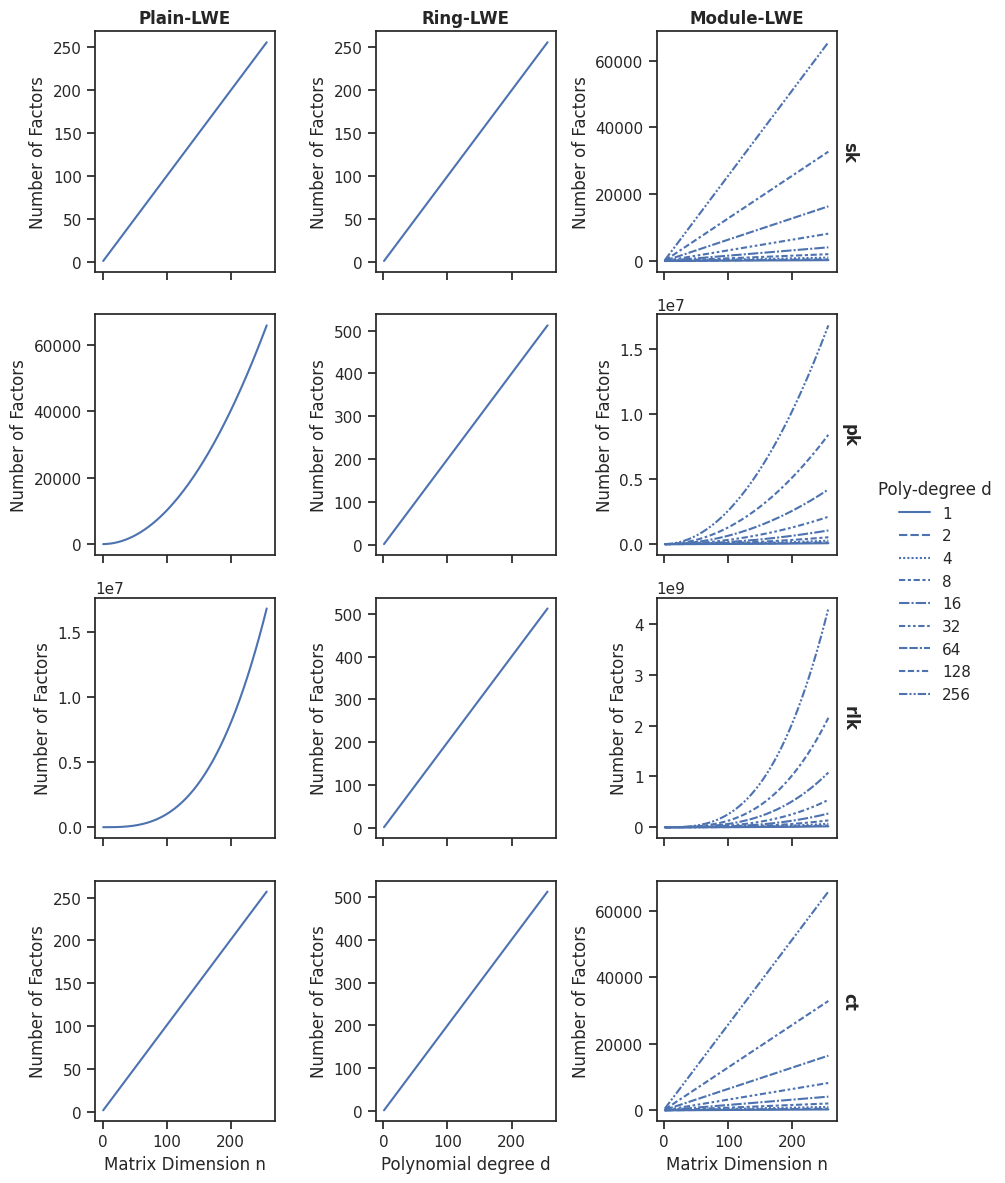
\includegraphics[scale=0.585]{images/OutputFactors.png}
  \caption[Output Variable Factors by Scheme]{The graph illustrates the growth in the number of factors (y-axis) against the dimensions (x-axis). Each of the three columns of plots represents a distinct scheme, as indicated at the top of the figure. The rows represent the output variables, which are indicated on the right-hand side of the right plot. In Plain-LWE and M-LWE, the x-axis is represented by the variable $n$. In contrast, R-LWE employs the variable $d$. In the case of M-LWE, the diverse line types serve to differentiate between distinct values of $d$.}
  \label{fig:OutputFactors}
\end{figure}

The growth rates observed for the secret key $sk$ are linear with regard to the variables $n$ and $d$ for Plain-LWE and R-LWE, respectively. M-LWE exhibits a linear relationship with either $n$ or $d$. When both variables grow simultaneously, the growth rate becomes quadratic. As a consequence, the growth rate for the number of factors in this case exhibits a significantly higher rate of increase than that observed for the other two schemes.

The linear growth rate observed for the $sk$ in R-LWE remains for both the private key $pk$ and the relinearization key $rlk$, but with an steeper incline. In contrast, the growth rates for the other two schemes exhibit a significant increase, particularly with regard to the matrix dimension $n$. For Plain-LWE the growth rate of the private key $pk$ is quadratic, while for the relinearization key $rlk$, it is even cubic. When increasing the polynomial degree $d$ simultaneously, the growth rate for M-LWE becomes cubic or quartic, respectively. It is also noteworthy that the $rlk$ does not employ the conventional modulus $q$, as all the other parameters do, but rather the larger modulus $q\cdot p$. As both moduli are represented in the computer as binary numbers, the maximum space they require can be expressed as $2^{q_b}\cdot 2^{p_b} = 2^{q_b+p_b}$. Therefore, rather than requiring $q_b$ bits, it is necessary to use $q_b+p_b$ bits to represent each factor for the $rlk$. This contributes to the unfavorable growth rates observed in Plain-LWE and M-LWE, as more and significantly larger numbers are needed.

The ciphertext $ct$ exhibits a similar growth pattern to that of the secret key $sk$. For Plain-LWE and M-LWE, the growth behavior is nearly identical, with the sole distinction being that, rather than $n$, $n+1$ is utilized. This is negatable when $n$ is increasing. As $n=1$ for R-LWE, the increment of $1$ results in a doubling of the requisite number of parameters, thereby causing the incline to double, but the growth rate remains linear.

One important note that need to be done, is the difference between word-wise and bit-wise FHE schemes \cite{WordBitWiseFhe}. The difference is, that bit-wise FHE operates at the single bit level and word-wise FHE operates on the whole word (eg, 64 bit). This means that each polynomial can be seen as a word and operations can be done all at once and the polynomial dimension $d$ defines the word size. For a bit wise scheme, the logic needs to be done bit wise, which means that a lot more operations need to be done, which makes bit-wise slower. In this thesis, BFV was chosen as backbone for the created M-LWE HE scheme, which is a word-wise scheme, but by choosing $d=1$ it is essentially turned into a bit-wise scheme. In practical terms, this implies that R-LWE and M-LWE are capable of encrypting an entire word at once, for example, 32- or 64-bit numbers. In contrast, Plain-LWE requires that each bit be encrypted individually. This necessitates the decomposition of words into their constituent bits, followed by their encryption and the construction of operations based on these single-bit ciphertexts. This approach not only demands greater computational resources but also requires more space for storing the additional data. Further advantages and disadvantages are detailed in reference \cite{WordBitWiseFhe}. 

In general, R-LWE requires the fewest number of factors and the smallest amount of physical space to store its output variables. In comparison, Plain and especially M-LWE require a greater number of factors and a greater amount of physical space. Furthermore, the growth rate for R-LWE is significantly lower than that of Plain and M-LWE. In defense of M-LWE, it should be noted that in practice the matrix dimension $n$ is quite small. In the CRYSTALS-Kyber scheme \cite{CyrstalsKyber}, the values are set between 2, which corresponds to low security, and 4, which corresponds to high security. This can be achieved because the security of the system is not solely dependent on the matrix, but also on the polynomials. In contrast to Plain-LWE, significantly larger values of $n$ are required for security. In the Frodo encryption scheme \cite{frodo}, which utilize Plain-LWE, values between $352$ for low security and $864$ for high security and a value of $n=752$ is recommended. This results in the number of factors exceeding $400$ million just for the $rlk$.

A comparison of the physical space required for the various encryption schemes, with variables based on the regular/recommended security level of published encryption schemes that employ the underlying method, can be found in Table \ref{table:OutputVariableInKB}. It is important to note that the results should be interpreted with caution and that direct comparisons between the numbers are not possible. However, the data provides a general indication of the differences between the schemes. Notably, the variables for Plain-LWE are considerably larger than those for the other two, requiring more than $3$ gigabytes, solely for the $rlk$. Even tho the ciphertext $ct$ is the smallest for Plain-LWE, this amount of disk space is necessary for each bit, whereas R-LWE and M-LWE can store $512$ or $256$ bits, respectively, with a slightly larger $ct$. With the exception of the ciphertext, R-LWE has the smallest overall size for every variable. However, as it can store twice the information of M-LWE and, as previously mentioned, $512$ times more than Plain-LWE, it requires the smallest amount per bit stored.

\begin{table}[htp]
  \centering
  \caption[Theoretical LWE HE output variable sizes]{Theoretical LWE Output Variable size in Kilobyte (KB), based on variables for the regular/recommended security level of published encryption schemes. The modulus $p=q^3; p_b=q_b*3$ as described in BFV}
  \begin{tabular}{|l|c||c|c|c|c||c|c|c|c|}
    \toprule
              & Source                      & $n$   & $d$   & $q$     & $q_b$ & $sk$   & $pk$      & $rlk$     & $ct$   \\
    \midrule
    Plain-LWE & \cite{frodo}                & $752$ &       & $32767$ & $15$  & $1.41$ & $1061.73$ & $3193684$ & $1.41$ \\
    R-LWE     & \cite{PracticalKeyExchange} &       & $512$ & $25601$ & $15$  & $0.96$ & $1.92$    & $7.68$    & $1.92$ \\
    M-LWE     & \cite{CyrstalsKyber}        & $3$   & $256$ & $7681$  & $13$  & $1.25$ & $4.992$   & $59.904$  & $1.66$ \\
    \bottomrule
  \end{tabular}
  \label{table:OutputVariableInKB}
\end{table}

In conclusion, the comparison based on the size of the output values indicates that R-LWE has the slowest growth of physical space needed based on its dimension variables. Although M-LWE has the fastest growth rate, as it is based on multiple dimension variables, this makes it far more secure than Plain-LWE. Consequently, the dimensions can be smaller in general to achieve a similar level of security, which results in a smaller physical size of its output variables. In terms of storage requirements for the output variables, Plain-LWE is by far the most demanding, with M-LWE requiring more physical space than R-LWE, except for the ciphertext. However, the difference in these requirements is not as significant as that observed in the comparison with Plain-LWE.

\section{Time cost comparison}

The objective of this section is to perform a comparative analysis of the runtime performance of the algorithms with respect to a selected set of input parameters. To minimize the impact of noise, multiple iterations of each algorithm were executed with the same inputs, and the median time value in seconds was calculated. In total, there are four parameters that can be modified: the dimensions $n$ and $d$, as well as the modulus values $q$ and $p$. To simplify the analysis of multiple variables and enhance the visualization of the differences, two performance tests were conducted. One test was conducted with varying dimension variables $n$ and $d$, while the modulus values $q$ and $p$ were constant. The second test was performed with the variables $n$ and $d$ fixed while the modulus values $q$ and $p$ were varied. This should provide a more straightforward means of illustrating the impact of these variables on the performance of the algorithms. The algorithms that are evaluated are the \textit{KeyGen} (Algorithm \ref{alg:HomomorphKeyGen}), the \textit{Encryption} (Algorithm \ref{alg: SampleLweEncryption}), the \textit{Decryption} (Algorithm \ref{alg: SampleLweDecryption}), the \textit{Addition} (Algorithm \ref{alg:MlweAddition}) and the \textit{Multiplication} (Algorithm \ref{alg:moduleMultiplication}).

The initial comparison is that of processing time, based on the two size dimensions, namely, $n$ and $d$. The results of the comparative analysis of the algorithms' performance are presented in Figure \ref{fig:nd-performance}. 

\begin{figure}[htp]
  \centering
  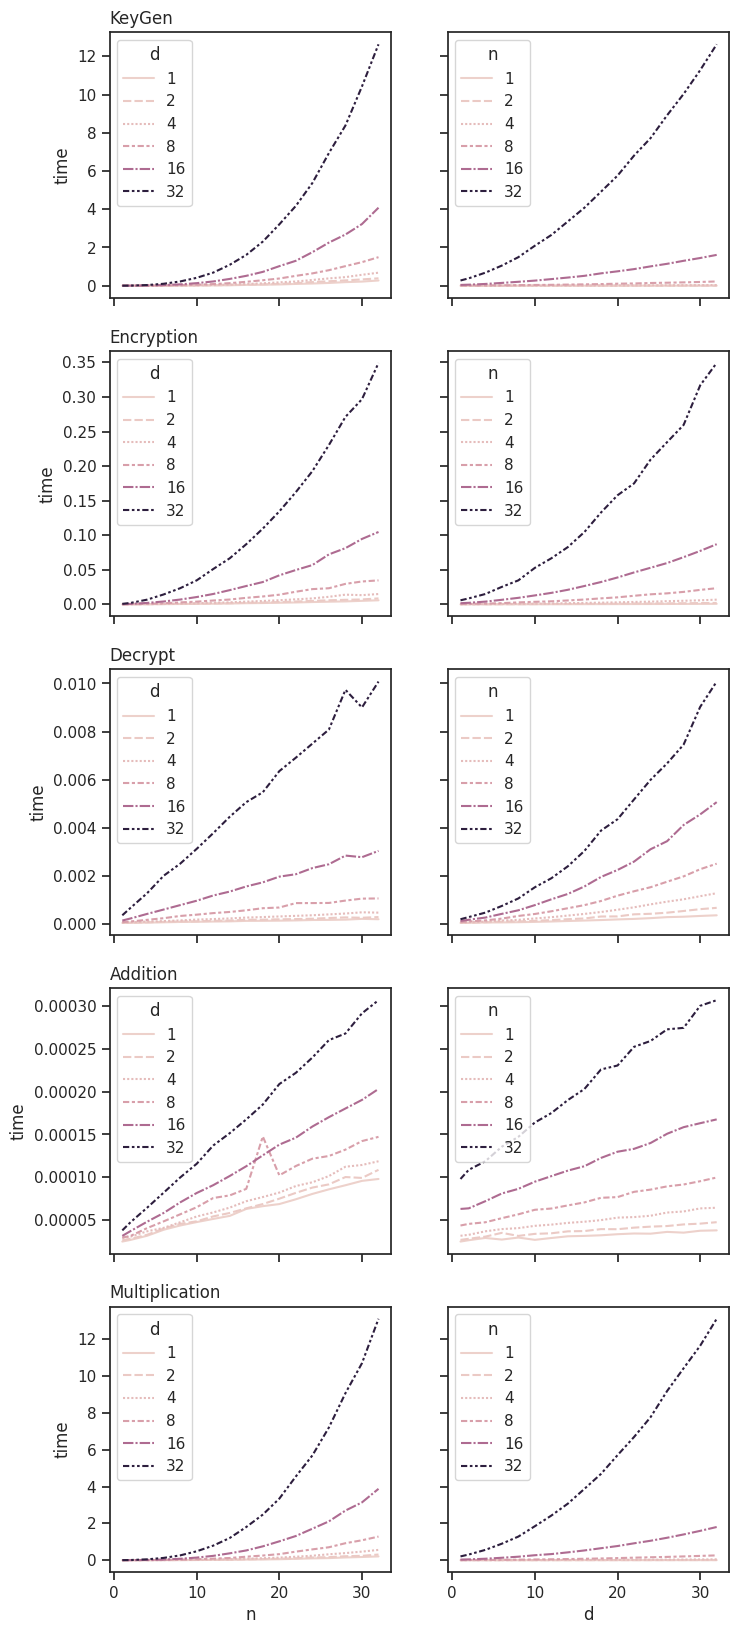
\includegraphics[scale=0.54]{images/nd-performance.png}
  \caption[Performance of the HE algorithms by $n$ and $d$]{Performance of the main algorithms in regard to dimensions $n$ and $d$ and the time in seconds. Each row is a different algorithm, as stated always above the left plot. The left column plots the time against $n$ for some $d$ values. The right column plots the time against $d$ for some $n$ values.}
  \label{fig:nd-performance}
\end{figure}

In the figure, Plain-LWE is illustrated in the left column, in the line representing $d=1$, and R-LWE is shown in the right column with $n=1$. All other lines represent distinct versions of M-LWE. It can be observed that the \textit{KeyGen} and \textit{Multiplication} algorithms are the most time-consuming. Regardless of whether $n$ or $d$ is increased, these algorithms exhibit an exponential growth in time cost. However, the rate of increase for $d$ is relatively modest, in contrast to the significant rise observed in the case of $n$. This exponential growth can be attributed to the fact that, in order to perform matrix multiplication, the number of scalar multiplications increases quadratically. One potential solution to this issue is the use of dedicated matrix multiplication hardware, which performs the entire operation in a single step, or the incorporation of other optimized libraries. But, as it was necessary to work with numbers larger than 64 bits, it was not possible to use such libraries in the implemented system. These optimized libraries (such as numpy) only support 64-bit integers in python. Therefore, the arbitrary size integers in pure Python were used and a simple matrix multiplication algorithm was created, which is not optimized. This provides an explanation as to why the increase of $n$ results in exponential growth, but also demonstrates that this phenomenon occurs at a slower rate when $d$ is increased and $n$ stays fixed. The rationale behind this is that, in order to perform polynomial multiplication, the methodology outlined in Section \ref{sec:PolyMulMath} was employed, which translates polynomial multiplication into matrix-vector multiplication. As the value of $d$ increases, the dimensions of the matrix also increase, resulting in a quadratic growth in the number of multiplications required, following the same pattern previously described. The combination of these two facts also explains why the growth for $n$ is more pronounced. In addition to the increase in the number of polynomial multiplications due to the larger dimensions, each new polynomial multiplication also exhibits a quadratic runtime.
As the number of matrix multiplications increases, the algorithms become less efficient, exhibiting a decline in speed. This phenomenon is most evident in the \textit{KeyGen} and \textit{Multiplication}, where a single matrix multiplication is required for each $rlk$, which increases linearly with $n$. Consequently, these algorithms are quite slow. The \textit{Encryption} algorithm requires only a single matrix-vector and one vector-vector multiplication, resulting in a quadratic growth rate. This makes it significantly faster than the previously mentioned algorithms. In contrast, \textit{Addition} does not require any multiplication, making it the fastest algorithm by far. As only vectors need to be added, the time growth is also linear, as the number of additions scales linearly with the size of the vectors. With the \textit{Decryption}, there is a very interesting pattern. While the runtime scales linearly with the increase of $n$, it has a quadratic growth with the increase of $d$. This is due to the quadratic scaling of the matrix required for the polynomial multiplication, as previously explained. \\
In consideration of the overall performance, the impact of the dimensions can result in a significant decline in performance, potentially by a factor of multiple and even orders of magnitude. Therefore, $n$ and $d$ exert a considerable influence on the performance.

\begin{figure}[htp]
  \centering
  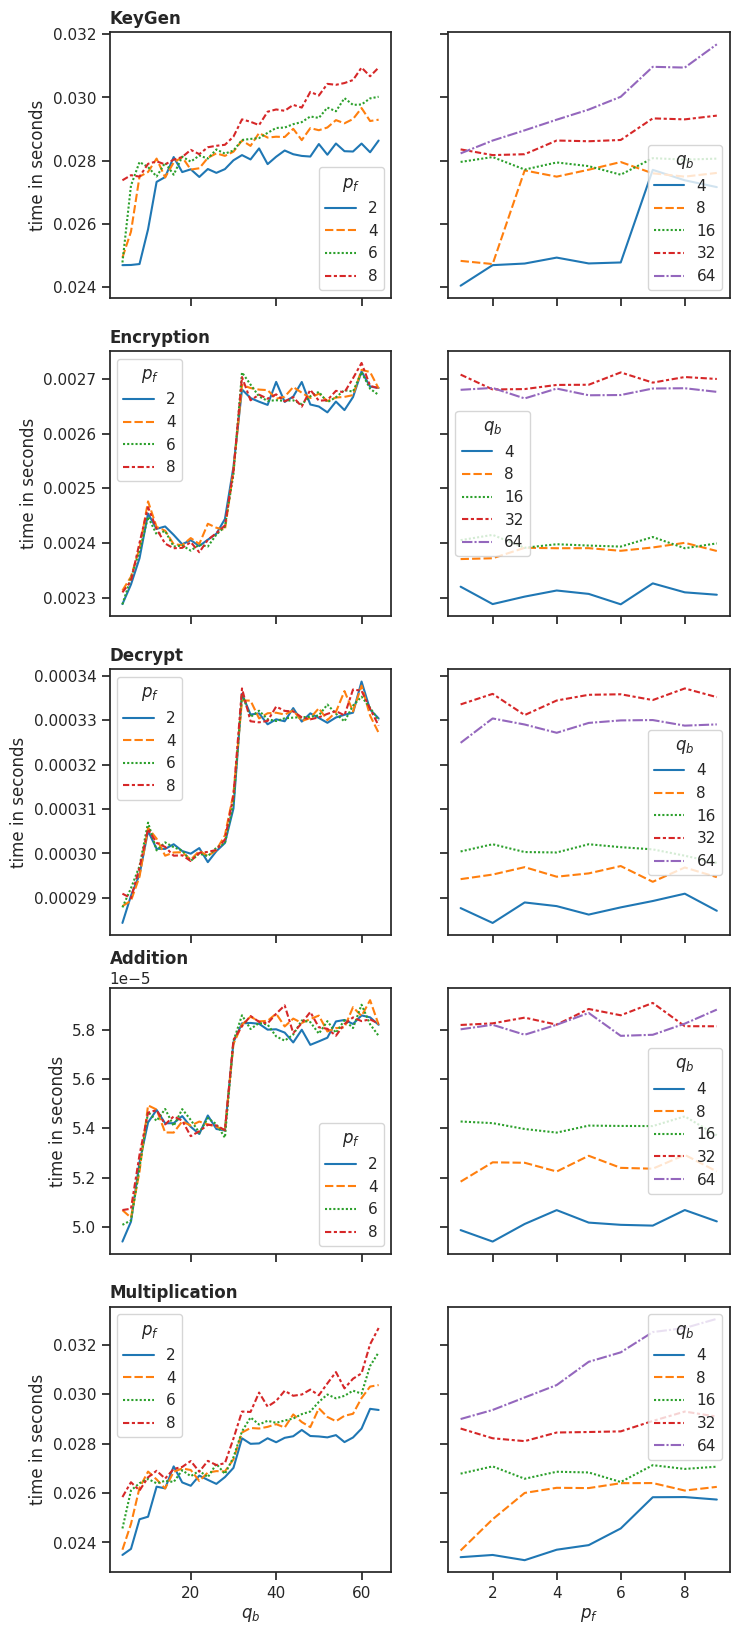
\includegraphics[scale=0.53]{images/qp-performance.png}
  \caption[Performance of the HE algorithms by $q_b$ and $p_f$]{Performance of the main algorithms in regard to modulus with $q_b$ bit and the modulus factor $p_f$, which represents $q_b\cdot p_f$ bit in regards to the time in seconds. Each row is a different algorithms, as stated always above the left plot. The left column plots the time against $q_b$ for some $p_f$ values. The right column plots the time against $p_f$ for some $q_b$ values.}
  \label{fig:qp-performance}
\end{figure}

The second cost comparison is based on the development of the modulus $q$ and $p$, as illustrated in Figure \ref{fig:qp-performance}. 
The quantity represented by the variable $q_b$ in the graph is the number of bits for the modulus $q = 2^{q_b}$, while the quantity represented by the variable $p_f$ is the factor by which the $q$ bits are multiplied to retrieve the modulus $p = 2^{q_b \cdot p_f}$. The rationale for this is that the value of $p$ should be a multiple of several orders of magnitude greater than that of $q$, as outlined in the BFV paper. Since the x-axis plots the $q_b$ or $p_f$ factors, the axis uses a logarithmic scale with respect to the actual modulus values.

Upon examination of the data, it becomes evident that there are two distinct groups of algorithms: KeyGen+Multiplication and Encryption+Decryption+Addition. The former exhibits a linear increase in time consumption, while the latter displays a pattern of steps and a constant time consumption between steps, as $q_b$ increases. The primary distinction between these two groups is that the former requires the use of $p$ for computations, whereas the latter employs solely $q$.  This is also the reason why, for the right graphs associated with group one, there is a linear increase with the increase of $p$, whereas for group two, this value remains constant. Group two, on the left side, exhibits performance jumps around $16$ and $32$ bits. It is plausible that Python has internal improvements for $16$ and $32$ bit numbers. However, this is not observed in the first group, as they calculate with numbers greater than $32$ bits due to the usage of $p$.

In general, it can be observed that the variables $q$ and $p$ exert a relatively minor influence on performance, particularly in comparison to the dimension variables. As evidenced by the data, even a significant discrepancy in $q$ and $p$ only results in a $40\%$ increase in the time required for multiplication. Especially, when considering the range of $p$ values, from $1 \cdot 4=4$ bits to $64 \cdot 8=512$ bits, which is an increase by factor $128$.



To provide some real-world examples, the same parameters as in the previous section (see Table \ref{table:OutputVariableInKB}) were used to calculate the performance in seconds, which can be seen in Table \ref{table:performanceComparison}. The Plain-LWE version was excluded from the comparison due to the discrepancy between the required memory and the available memory, which prevented its execution. Even if the limitation could be overcome, the runtime would be significantly slower than that observed for the other two versions. A comparison of the two other two schemes reveals that they both operate within the same order of magnitude. With the exception of the decryption algorithm, the R-LWE algorithms are consistently faster than their M-LWE counterparts. This discrepancy in decryption time may be attributed to the fact that R-LWE has twice the polynomial degree $d$, compared to M-LWE. But this also means, that R-LWE works with the double word size at the same time, which allows for bigger numbers to be operated on. Additionally, it is not unexpected that the M-LWE version is slower than R-LWE, as the higher matrix dimension, $n$, necessitates more calculations.

\begin{table}[htp]
  \centering
  \caption{M-LWE and R-LWE Performance in seconds, based on variables for the regular/recommended security level of published encryption schemes}
  \begin{tabular}{|l|c||c|c|c|c|c|}
    \toprule
          & Source                      & Addition & Decrypt  & Encryption & KeyGen   & Multiplication \\
    \midrule
    R-LWE & \cite{PracticalKeyExchange} & 0.000163 & 0.061521 & 0.125041   & 0.182526 & 0.473052       \\
    M-LWE & \cite{CyrstalsKyber}        & 0.000176 & 0.041224 & 0.174293   & 0.696122 & 1.039662       \\
    \bottomrule
  \end{tabular}
  \label{table:performanceComparison}
\end{table}

As previously demonstrated, the majority of algorithms exhibit a quadratic growth in runtime with respect to the dimension variables, namely $n$ and $d$. This is growth rate is especially problematic for KeyGen, which has the advantage of being executed only once per session, and for multiplication, which is a significant challenge for homomorphic encryption schemes. In order to maintain satisfactory performance, it is advisable to minimise the dimensions, with particular attention paid to the matrix dimension $n$, which exhibits a higher growth rate and therefore a greater influence. In contrast, the influence of the modulus $q$ and $p$ on performance is comparatively minor, particularly in comparison to the dimension variables. Thus, increasing these variables results in a slight decline in performance, but not a drastic one. When examining real-world parameters, it becomes evident that R-LWE remains the best choice, closely followed by its M-LWE counterpart. Plain-LWE exhibits a considerable memory footprint, which would also result in a significant decline in performance, rendering it impractical to run this version at all in practice.

\section{Comparison of the additive and multiplicative depth}

As a last test, the additive and multiplicative depth of the LWE based HE schemes will be compared. As the number of operations performed in a homomorphic manner increases, the resulting error grows in magnitude. After a certain number of operations, the accumulated error becomes so significant that the decryption process yields incorrect numerical values. The source of the error is the ciphertext itself, which is the foundation of LWE's security. This section will examine the maximum depth and the extent of the error growth for addition and multiplication operations, as well as the impact of dimension variables $n$ and $d$, and modulus variables $q$ and $p$.

The following statistical data were derived from a process whereby an operation was performed repeatedly with on a random ciphertext. The initial step involved encrypting a randomly generated message, thereby creating the original ciphertext. In each iteration, a new, randomly generated message was encrypted, resulting in a new, second ciphertext. Subsequently, the new, second  ciphertext was added or multiplied, depending on the specific test, to the original message, thereby updating it. After that, the updated ciphertext was evaluated to ascertain whether the resulting message, obtained through decryption, exhibited the same outcome as if the calculations had been performed in plaintext space. The discrepancy between the present ciphertext and the correct plain text, the error, was recorded for each iteration.
This process is then repeated until either the decrypted message does not match the expected result or until a pre-defined maximum limit is reached, as otherwise the procedure would take an excessive amount of time. For each parameter set, this process was repeated multiple times to reduce noise. The median values for each round were then calculated. The rounds are referred to as depth, which denotes the number of consecutive operations that can be performed.

\begin{figure}[htp]
  \centering
  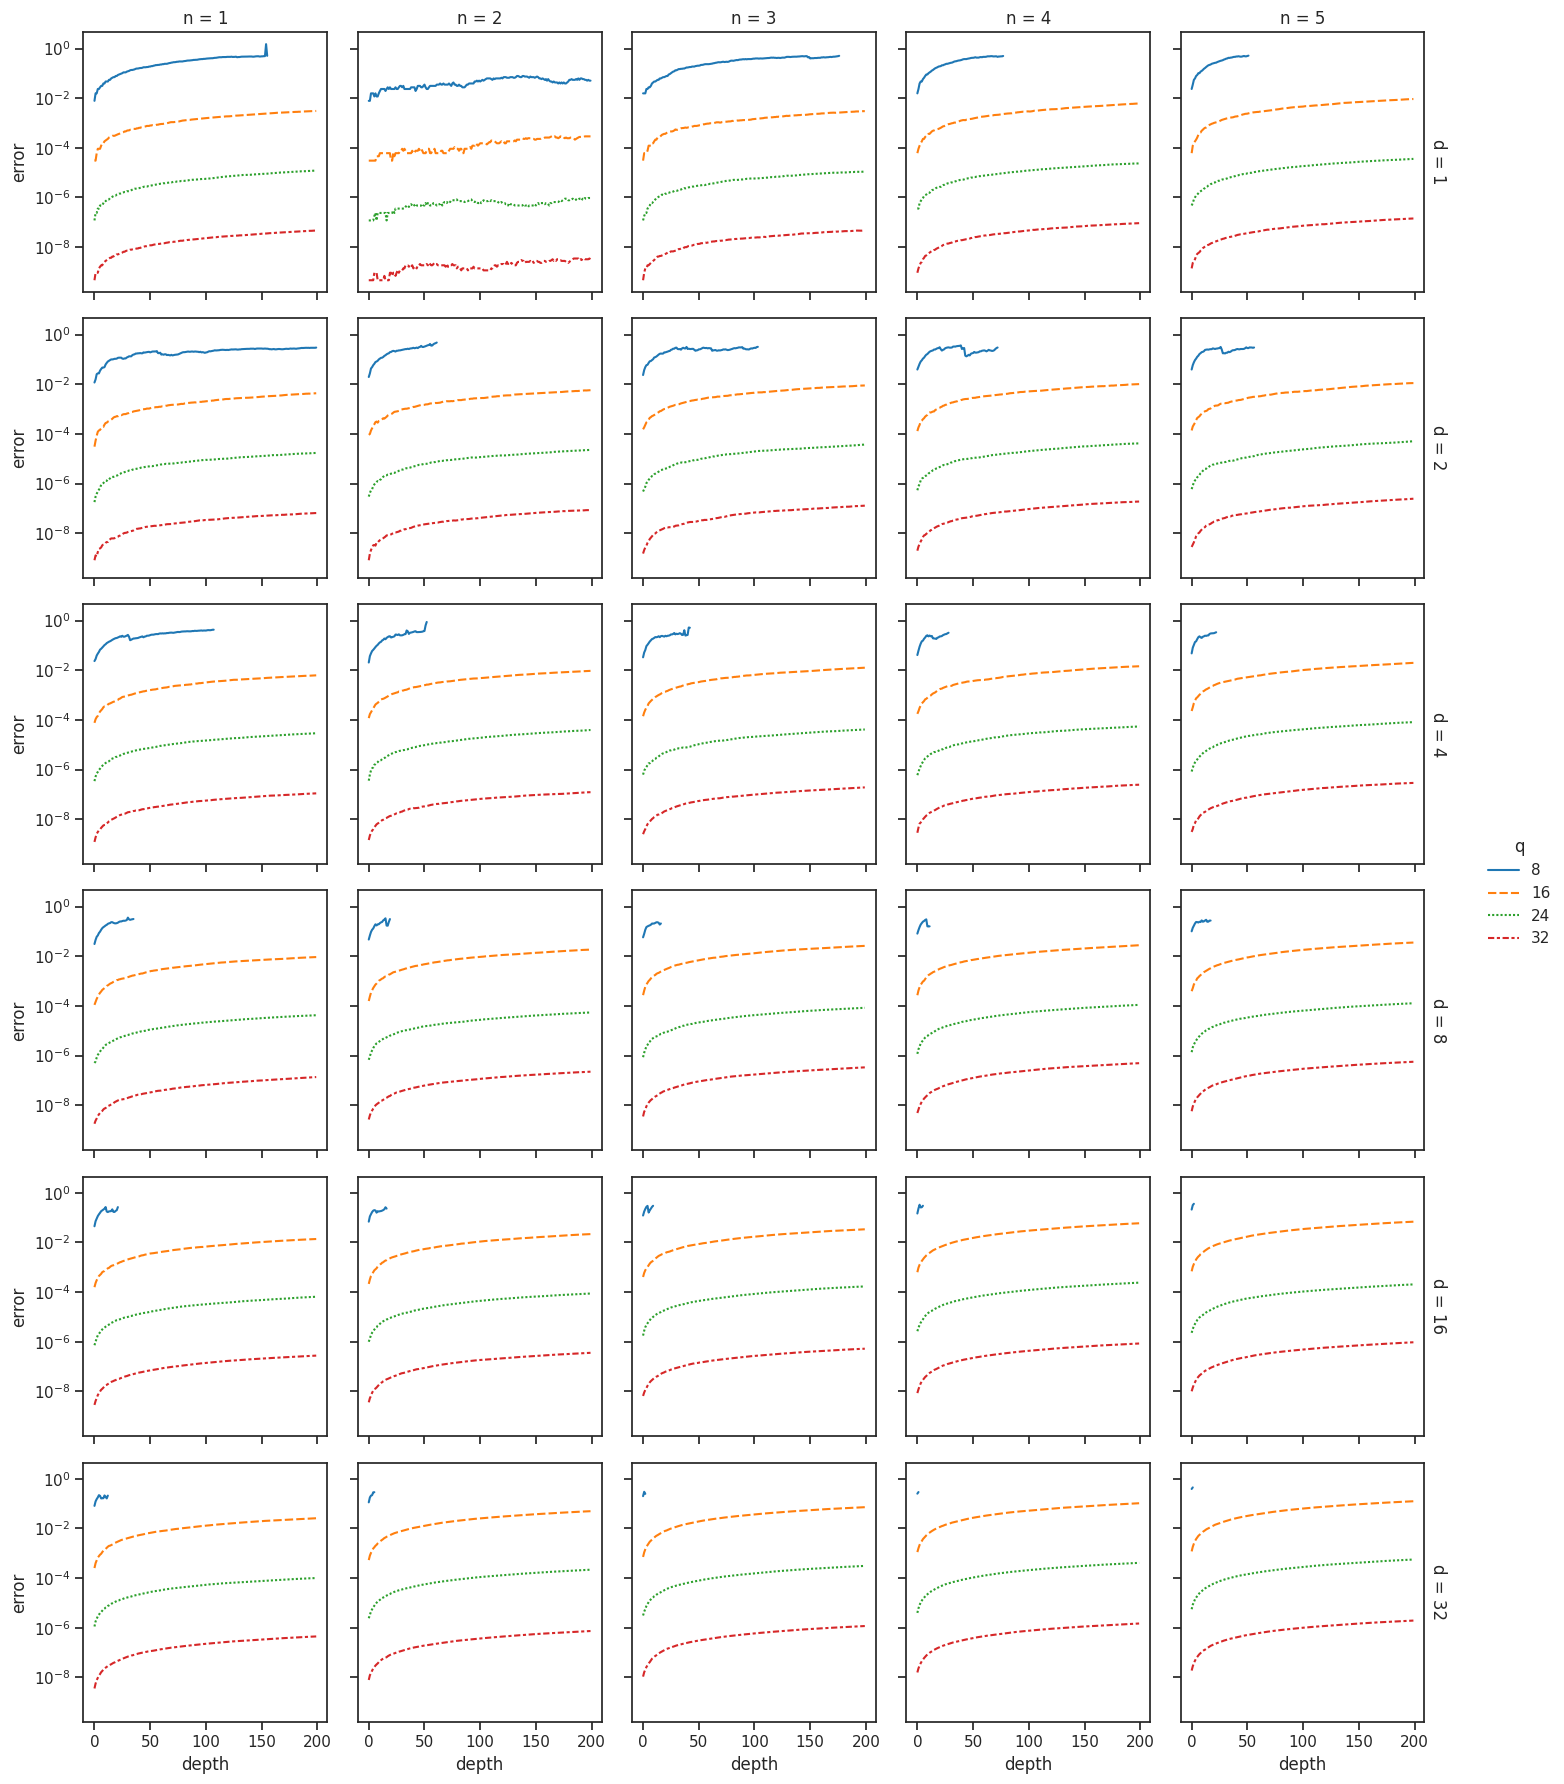
\includegraphics[scale=0.4]{images/AddErrorDevelopment.png}
  \caption[Additive Error Development]{Additive Error Development}
  \label{fig:AddErrorDev}
\end{figure}

First, the additive depth and error will be subjected to examination. The graphs illustrating this can be seen in Figure \ref{fig:AddErrorDev}. The addition is dependent on three variables: the two dimensional variables and the modulus, $q$. The modulus $p$ is not a required component of the addition process and therefore does not exert any influence on it. The figure illustrates the evolution of the error with depth for various configurations of the dimensions and for different modulus values. Once more, the value of $q_b$ represents the exponent, and the utilized modulus is defined as $q = 2^{q_b}$. The error axis is logarithmic in order to facilitate the visualization of the comparative magnitude of the errors. A logarithmic curve is observed in nearly all of the graphs, indicating that the error grows in a linear fashion with depth. In the event that the value of $q$ is insufficient, the curve will be terminated prematurely, as the resulting error is too high for successful decryption. As the value of $q_b$ increases, the minimum error decreases, thereby enabling a greater number of operations. However, when $n$ or $d$ are increased, the minimum error rises due to the number of total factors and with that more error in the system. Accordingly, as the dimensions increase, a larger modulus must be selected to facilitate subsequent additions. The linear growth can be attributed to the fact that the errors resulting from the addition are simply added together, as outlined in algorithm \ref{alg:MlweAddition}. Therefore, the resulting error is equal to the sum of the two errors from the ciphertexts. In this experiment, only freshly encrypted data with a minimal error was added to one ciphertext. In practice, however, ciphertexts with larger errors will also be added, as they will have undergone previous operations. When the errors are combined, the growth rate will be faster than that shown in the graph. Nevertheless, the growth rate remains linear and thus manageable with a sufficiently large modulus. This makes it possible to run more then $200$ additions easily, as can be seen by the error in the graphs. Also the maximum used modulus with $q = 2^{32}$, is not that high and bigger ones could be used without any problem making it possible to run many more additions in a row.

A comparison of the various LWE schemes reveals that the difference in computational depth for addition is not significant when evaluated based on depth alone. A comparison of the associated data indicates that the variables $n$ and $d$ exert a comparable influence on the reduction of computation depth. Consequently, an evaluation of the graphs suggests that Plain-LWE (first row) and R-LWE (first column) exhibit comparable performance for small dimensions. M-LWE, however, which incorporates both $n$ and $d$ into its formulation,results in a lower computational depth for addition.

The next step is to analyse the multiplication process, which is illustrated in Figure \ref{fig:MulErrorDev}. The multiplication function makes use of the modulus $p$ for the modulus switching component. The impact of this variable is illustrated by the colored bands displayed alongside each graph. It displays the minimum to maximum error values for all values of $p$ at that depth. To obtain a comprehensive set of values, multiple runs were conducted with identical dimension variables and modulus and varying $p_f$ values between $1$ and $15$. These $p_f$ values were used to calculate the modulus $p=2^{q_b\cdot p_f}$. The primary line represents the median values for a given depth across all $p$ values.

\begin{figure}[htp]
  \centering
  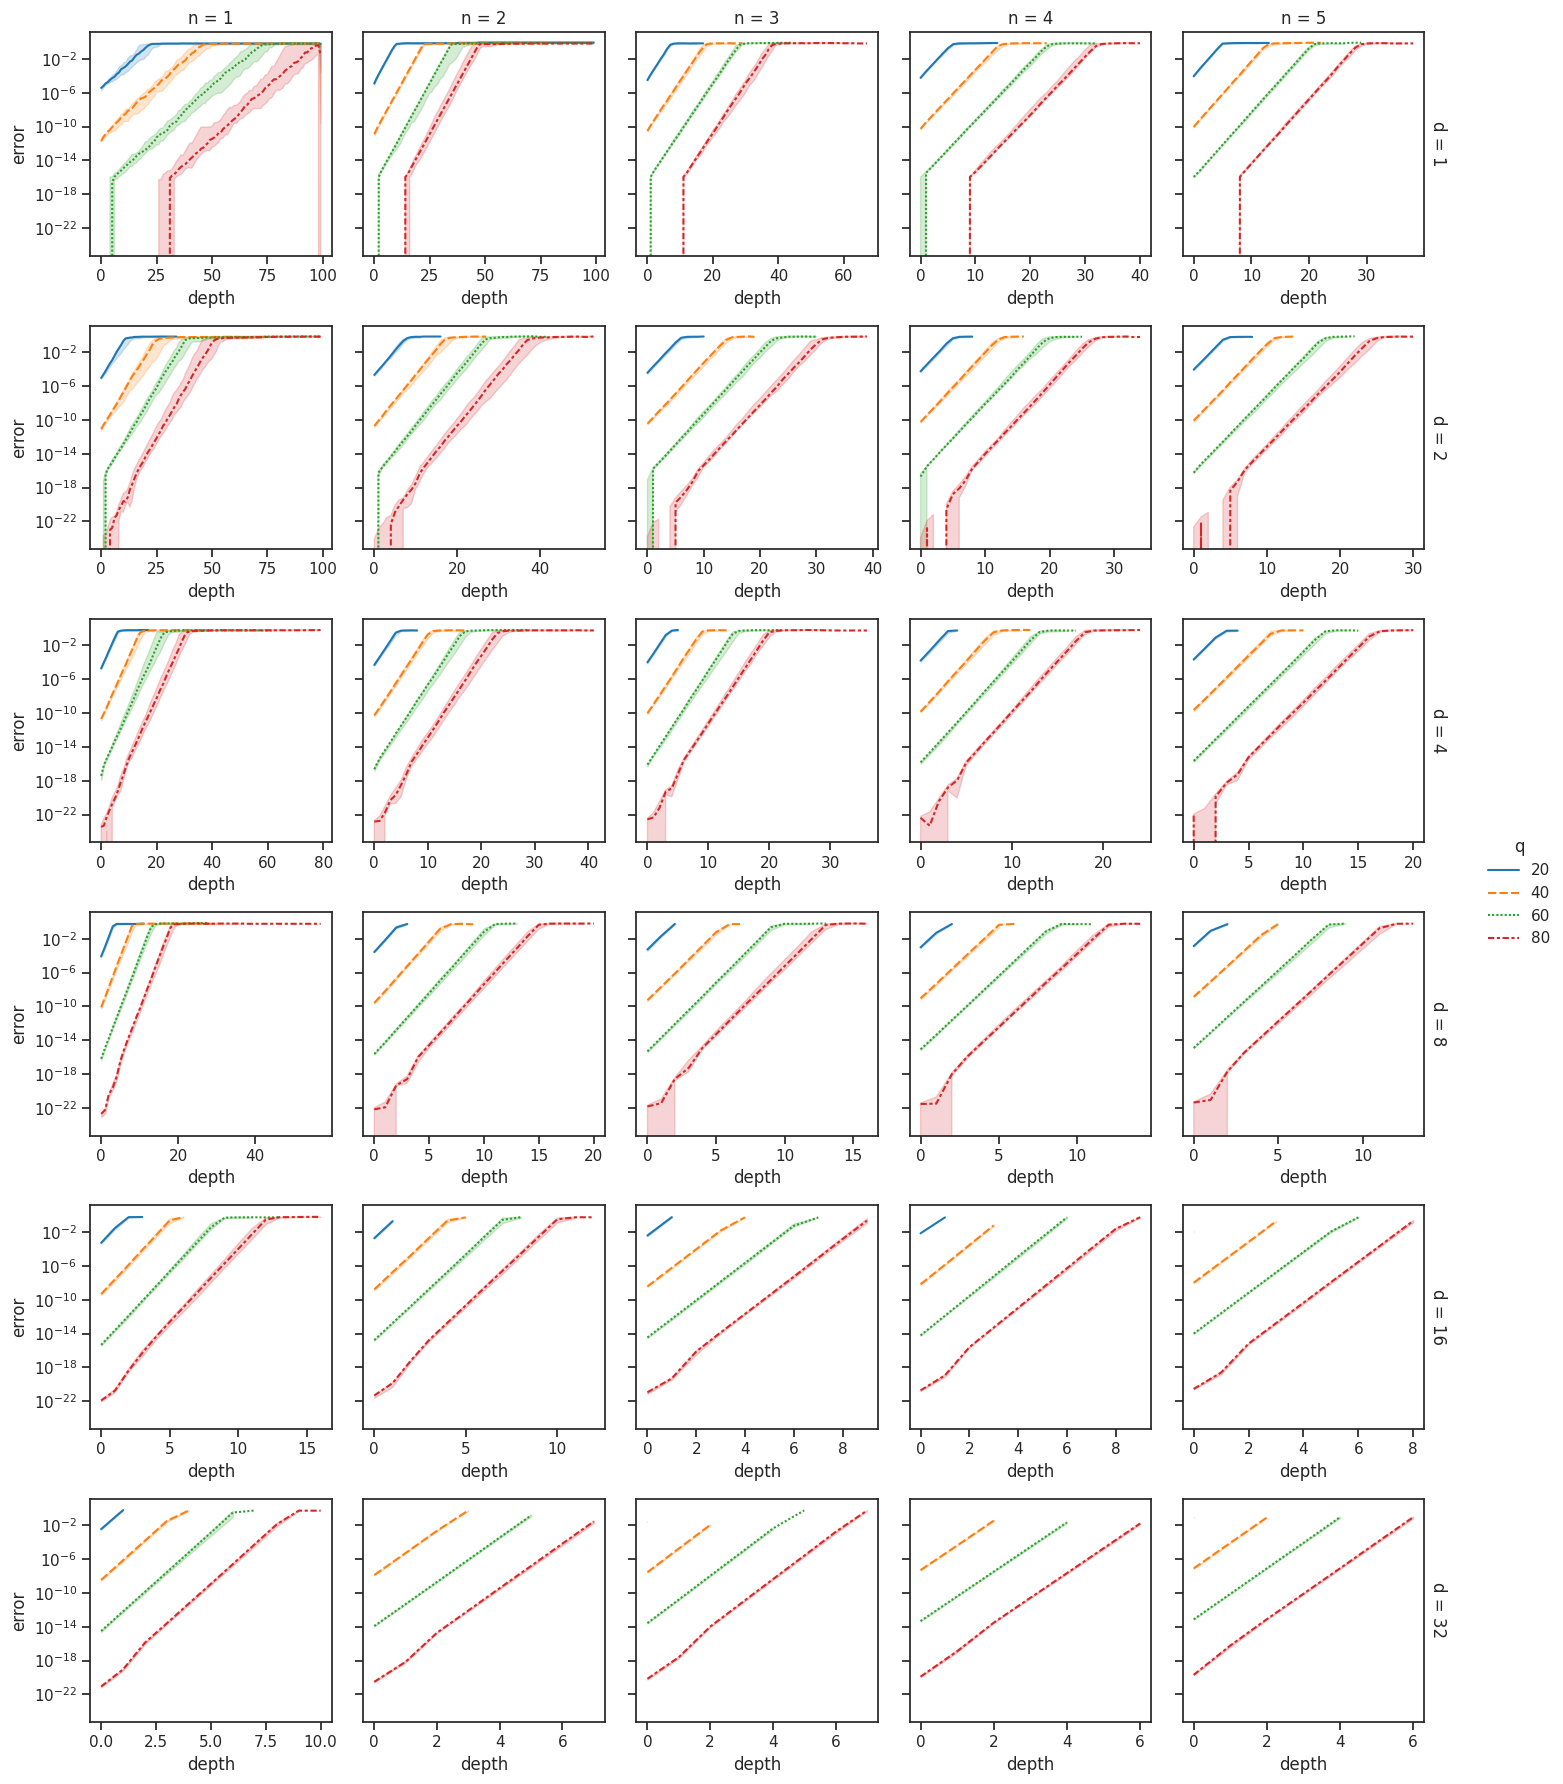
\includegraphics[scale=0.4]{images/MulErrorDevelopment.png}
  \caption[Multiplicative Error Development]{Multiplicative Error Development}
  \label{fig:MulErrorDev}
\end{figure}

In contrast to the behavior observed in the addition function, the error line in these graphs is, in general, more linear. As the error axis employs a logarithmic scale, the error grows exponentially with each multiplication. This results in a relatively shallow depth, particularly when the dimensions are increasing. To illustrate, the maximum depth attained in the bottom rightmost graph is $6$, with an modulus of $q = 2^{80}$. The aforementioned error growth is also elucidated in other studies regarding LWE-based FHE schemes. For instance, in reference \cite{FHEwoBottstrapping}, it is detailed that the error for addition increases by a maximum of two, while for multiplication, the error is quadratic in the worst case. These analogous growth rates are observable in the graphs for addition and multiplication.

The value of $p$ is utilized for the modulus switching process, with the objective of enabling multiplication and concurrently reducing the error, as detailed in the BFV paper. As evidenced by the graphs, this objective was not achieved for any value of $p$. Furthermore, an additional trial was conducted, wherein the value of $p$ was increased to a considerably higher amount, specifically $1000$. This resulted in the generation of a modulus with a size of $2^{q*1000}$. However, this approach did not yield any apparent improvement in the outcomes observed for the higher-dimensional M-LWE schemes, such as the one depicted in the bottom right region of the graph. The precise reason why $p$ has no tangible impact is yet to be determined. One potential explanation for this discrepancy is the presence of numerical issues and minor rounding errors associated with the manipulation of these large numbers in Python. In particular, the process of dividing by $p$, as illustrated in steps $4$ and $5$ of algorithm \ref{alg:moduleMultiplication}, may introduce rounding errors due to the conversion from an arbitrary-size integer to a $64$-bit float. This could potentially contribute to the observed issue.

When comparing the influence of the variables $n$ and $d$ and, consequently, the various schemes, on the multiplication error and depth, it becomes evident that, as was the case with addition, both variables exert a roughly equivalent influence. Therefore, irrespective of the variable that is increased, the computational depth rate will decline to a similar extent. As observed in the case of multiplication and addition, by enhancing the modulus $q$, the minimum error can be lowered, consequently leading to an increase in the computational depth.

\begin{table}[htp]
  \centering
  \caption[M-LWE and R-LWE computation depth comparison]{A comparison of the computation depth of M-LWE and R-LWE for variable modules, with $q = 2^{q_b}$ and $p=2^{q_b\cdot 3}$. The remaining parameters are based on variables corresponding to the regular or recommended security level of published encryption schemes. The resulting numbers are the median values when an error occurred and thus no further calculations were possible.}
  
  \begin{tabular}{|cc|rrrrrr|rrrrrr|}
    \toprule
                                       &       & \multicolumn{6}{|c|}{Addition} & \multicolumn{6}{|c|}{Multiplication}                                                        \\
                                       & $q_b$ & 13                             & 15                                   & 20  & 32  & 64  & 128 & 13 & 15 & 20 & 32 & 64 & 128 \\
    \midrule
    R-LWE  \cite{CyrstalsKyber}        &       & -                              & 56                                   & 200 & 200 & 200 & 200 & -  & 0  & 0  & 1  & 3  & 7   \\
    M-LWE  \cite{PracticalKeyExchange} &       & 7                              & -                                    & 200 & 200 & 200 & 200 & 0  & -  & 0  & 1  & 3  & 7   \\
    \bottomrule
  \end{tabular}
  \label{table:depthComparison}
\end{table}

As a final comparative analysis, the R-LWE and M-LWE algorithms were once again evaluated with the aid of a number of recommended parameters. The outcome of this comparison is presented in Table \ref{table:depthComparison}. In order to evaluate the computational feasibility of the proposed approach, the experiment was conducted with increased modulus values. Both the M-LWE and R-LWE versions are capable of performing addition in their base configurations, however, the depth for the R-LWE is considerably higher than that for the M-LWE. This comes from the fact that in their base versions, the R-LWE version has a bigger modulus $q$ then the M-LWE version. However, it was not possible to perform multiplication for any scheme with the original modulus values. As the value of $q$ increased, the depth for addition could be easily raised to the maximum depth for this comparison ($200$) for both schemes in an equal manner. Achieving the desired increase in depth for multiplication proved more challenging. With a modulus of $128$-bits, only an average of seven computations in a row were feasible. However, the values observed between the models are identical, indicating that the error increase is approximately equivalent across both R-LWE and M-LWE. In general it can be seen, that the R-LWE and M-LWE schemes are quite similar in additive and multiplicative depth for the same modulus $q$.

As discussed before, with a polynomial dimension $d$ for R-LWE that is twice that of M-LWE, R-LWE is capable of processing significantly larger numbers.
\chapter{Conclusion}

The principal objective of this thesis was to investigate the viability of transferring R-LWE homomorphic encryption schemes to M-LWE and to evaluate the performance of these novel schemes. The viability of this approach was evaluated by developing an M-LWE HE scheme using the BFV scheme \cite{BFV}.
 
As detailed in Section \ref{sec:GeneralizingToMLWE}, it is possible to extend R-LWE-based HE schemes to M-LWE, thereby creating novel HE schemes where not only the polynomial rank $d$ but also the dimension size $n$ of the matrix can be modified. This also permits the creation of Plain-LWE HE schemes, as these are a special case of M-LWE, where $d=1$. To accomplish this, an M-LWE encryption scheme was extended to accommodate homomorphic  addition and multiplication operations. In the case of the addition operation, this was a trivial process, as the values could be added together in the same manner as was done previously with R-LWE. The process for multiplication is somewhat more cumbersome and comprises a greater number of steps. The primary challenge was the generation of an $n \times n$ matrix during the multiplication of the ciphertexts. Given that the resulting ciphertext must retain its original structure, comprising a polynomial and a vector of polynomials, this matrix must be decomposed and incorporated into the other values. By decomposing this matrix and multiplying it with $n$ relinearization keys, rather than a single one, the requisite output structure can be created, which, given a sufficiently large modulus $q$, will decrypt to the desired results. Given the general nature of the decomposition process, it seems reasonable to hypothesize that the same method could be applied with minor modifications to other R-LWE-based HE schemes.

% die höhere varianze durch mehr variablen, konnte nicht die fehlerrate senken, sondern

In examining the findings of the evaluation, it becomes evident that the M-LWE scheme exhibits both advantageous and disadvantageous characteristics. Prior to an in-depth examination of R-LWE and M-LWE, it is worthwhile to briefly consider the characteristics of Plain-LWE. It is evident that a homomorphic version based on BFV cannot be used to construct a secure encryption scheme with Plain-LWE. The primary challenge lies in the substantial memory requirements for the variables (see \ref{table:OutputVariableInKB}), particularly the relinearization key, which is significantly higher than what a practical implementation would allow. Even with future advancements in memory, networking for transmission, and computing power, the size will remain impractically large. Exchanging the key and performing operations with it will be computationally expensive, making it infeasible. This conclusion is particularly noteworthy given that the other two methods are perceived to be more effective.

A comprehensive assessment of R-LWE and M-LWE reveals that it is not a straightforward task to reach a definitive conclusion. A significant distinguishing factor between these two that merits consideration, particularly when evaluating practical encryption protocols, is the word size. This refers to the number of bits that each of the schemes is capable of encrypting and working with in a single operation. In the practical examples, R-LWE utilises a polynomial rank, that is equal to the word size, of $512$, while M-LWE employs a word size of $256$. As the majority of computations and data structures operate within a $32$- or $64$-bit system, these word sizes are the most relevant in practical applications. Even when larger numbers are employed, $256$- or $512$-bit numbers are uncommon. This raises the question of whether it might be advantageous to utilize smaller polynomial ranks and enhance security by scaling up the matrix dimension, $n$. This topic will be elaborated upon in the latter part of this conclusion.

Upon initial comparison of M-LWE and R-LWE based on their parameter sizes, R-LWE appears to exhibit superior characteristics. In contrast to M-LWE, the increase in parameters for R-LWE is always linear to the polynomial rank, $d$. Conversely, when the matrix dimension, $n$, is increased in M-LWE, the private key, $pk$, and the relinearization key, $rlk$, increase exponentially, resulting in a significant increase in memory consumption. 
In practice, smaller polynomial ranks are employed for M-LWE, however, this does not offset the growth in parameters resulting from higher matrix dimensions. This is evident from Table \ref{table:OutputVariableInKB}. The issue of the accelerated growth rate for the private key and the relinearization key is that these keys must be exchanged prior to the initiation of encrypted communication. Given a fixed speed and capacity of networks, the establishment of an encrypted channel is more time-consuming with M-LWE, as a greater volume of data must be transmitted. However, the ciphertext is smaller for M-LWE than for R-LWE, at least in practical analysis. This implies that, with sufficient data, the initial higher cost can be offset and potentially reduced over the course of communication, allowing for the storage of more data with the same amount of disk space. In an enterprise setting, this could enhance the viability of M-LWE over R-LWE. 

Another characteristic that seems superior in R-LWE in contrast to M-LWE is the processing time. As the calculations in R-LWE only depend on scalar polynomials, less operation need to be done compared to the vector and matrix processing of M-LWE. The big advantage of M-LWE is, that these matrix operations can easily run in parallel. So instead of running one big matrix multiplication, when multiplying two polynomials in R-LWE, multiple smaller matrix multiplications can run in parallel. For M-LWE the polynomial rank can also stay fixed and improving the security can be done purely by increasing the matrix dimension. Therefore optimized multiplications can be implemented based on this fixed size polynomials, instead of re-implementing optimized versions for the different R-LWE security levels based on different polynomial ranks. This matrix multiplication optimization has already be done for the Crystal Kyber encryption scheme \cite{CyrstalsKyber}, where hardware solutions have been constructed already (\cite{KyberHardware}, \cite{KyberHardware2}). If these can be reused this would create new synergies between different M-LWE based encryption schemes.

The depth of operations for both the tested R-LWE and M-LWE scheme appear to be essentially equivalent, as demonstrated in Table \ref{table:depthComparison}. It appears that the polynomial rank and matrix dimension exert a comparable influence on the outcome, suggesting that augmenting one while reducing the other results in outcomes that remain within a similar range. The most pronounced impact arises from the increase in modulus $q$, which is consistent across both versions.

One potential approach to enhancing the M-LWE HE scheme would be to optimize it by reducing the polynomial rank (thereby reducing the word size) and increasing the matrix dimension in a manner that minimizes the ciphertext size while maintaining the same security level and avoiding an excessive increase in memory size of the private key and relinearization key. This increases the number of matrix multiplications, but because of the smaller polynomial rank, these matrices are smaller. This could be used to run these calculations in parallel over multiple CPU cores or dedicated hardware like GPUs or TPUs, which are becoming increasingly accessible even in more affordable hardware, due to the advent of large language models.



% Probleme in der Arbeit
% Python macht rundungsfehler bei großen zahlen
% Security wurde komplett außer acht gelassen
% Die basis Version von BFV, ohne verbesserungen wurde verwendet, welche veraltet ist


% Future Work
% Making SWHE to FHE
% Analyzing security aspect in more detail
% Using different, more modern basis instead of BFV
% Trying improved implementation and maybe Hardware acceleration

% ===============
%  Verzeichnisse
% ===============

% Verzeichnisse mit einzeiligem Zeilenabstand
\singlespacing

% Literaturverzeichnis
\listofreferences

% Abbildungsverzeichnis einfügen
\listoffigures

% Tabellenverzeichnis einfügen
\listoftables

% Algorithmenverzeichnis einfügen
\listofalgorithms

% % Quelltextverzeichnis einfügen
% \listoflistings

% =========
%  Appendix
% =========

\begin{appendices}

  \chapter{Example Calculations}

\section{Example Multidimensional Ring Calculation}
\label{app:ExampleMultiRingCalc}

Consider the ring $R = \mathbb{Z}_5[x]/(x^3+1)$ and 
$$
  f =\begin{bmatrix}
    1+2x+3x^2 & 2+3x+4x^2 \\
    3+4x+x^2  & 1+3x+4x^2 \\
  \end{bmatrix} \in R^{2\times 2}
$$

$$
  g = \begin{bmatrix}
    1+x+x^2   \\
    2+2x+2x^2 \\
  \end{bmatrix} \in R^2
$$

\begin{align*}
  f \cdot g & = {
  \begin{bmatrix}
    1+2x+3x^2 & 2+3x+4x^2 \\
    3+4x+x^2  & 1+3x+4x^2 \\
  \end{bmatrix}
  \cdot
  \begin{bmatrix}
    1+x+x^2   \\
    2+2x+2x^2 \\
  \end{bmatrix}
  }               \\
            & = {
  \begin{bmatrix}
    \begin{bmatrix}
      1 & -3 & -2 \\
      2 & 1  & -3 \\
      3 & 2  & 1  \\
    \end{bmatrix} & 
    \begin{bmatrix}
      2 & -4 & -3 \\
      3 & 2  & -4 \\
      4 & 3  & 2  \\
    \end{bmatrix}   \\
    \begin{bmatrix}
      3 & -1 & -4 \\
      4 & 3  & -1 \\
      1 & 4  & 3  \\
    \end{bmatrix} & 
    \begin{bmatrix}
      1 & -4 & -3 \\
      3 & 1  & -4 \\
      4 & 3  & 1  \\
    \end{bmatrix}   \\
  \end{bmatrix}
  \cdot
  \begin{bmatrix}
    \begin{bmatrix}
      1 \\
      1 \\
      1 \\
    \end{bmatrix} \\
    \begin{bmatrix}
      2 \\
      2 \\
      2 \\
    \end{bmatrix} \\
  \end{bmatrix}
  }               \\
            & = {
  \begin{bmatrix}
    1 & -3 & -2 & 2 & -4 & -3 \\
    2 & 1  & -3 & 3 & 2  & -4 \\
    3 & 2  & 1  & 4 & 3  & 2  \\
    3 & -1 & -4 & 1 & -4 & -3 \\
    4 & 3  & -1 & 3 & 1  & -4 \\
    1 & 4  & 3  & 4 & 3  & 1 
  \end{bmatrix}
  \cdot
  \begin{bmatrix}
    1 \\
    1 \\
    1 \\
    2 \\
    2 \\
    2 
  \end{bmatrix}
  }               \\
            & = {
  \begin{bmatrix}
    -14 \\
    2   \\
    24  \\
    -14 \\
    6   \\
    24
  \end{bmatrix}
  \mod 5
  }
  = {
  \begin{bmatrix}
    1 \\
    2 \\
    4 \\
    1 \\
    1 \\
    4
  \end{bmatrix}
  }
  = {
  \begin{bmatrix}
    \begin{bmatrix}
      1 \\
      2 \\
      4
    \end{bmatrix} \\
    \begin{bmatrix}
      1 \\
      1 \\
      4
    \end{bmatrix} \\
  \end{bmatrix}
  }               \\
            & = {
  \begin{bmatrix}
    1+2x+4x^2 \\
    1+1x+4x^2
  \end{bmatrix}
  }
\end{align*}


\section{Plain LWE}
\label{app:PlainLweCalc}
The following calculations should show the working of the Plain LWE encryption for the algorithms \ref{alg: SampleLweKeyGen} to \ref{alg: SampleLweDecryption}. The ring used for this calculations is defined as $R=\mathbb{Z}_{100}$ and $n=2$ for the dimensions. Starting first with the key generation:


\begin{align*}
  s  & = \begin{bmatrix}1 \\ 2 \end{bmatrix}
  A  = \begin{bmatrix}56 & 77 \\ 29 & 59 \end{bmatrix}
  e  = \begin{bmatrix}99 \\ 1 \end{bmatrix}       \\
  b  & = As+e                                     \\
     & = \begin{bmatrix}
           56 & 77 \\
           29 & 59
         \end{bmatrix}
  \cdot
  \begin{bmatrix}
    1 \\
    2
  \end{bmatrix}
  +
  \begin{bmatrix}
    99 \\ 
    1 
  \end{bmatrix}
  \\
     & = 1
  \cdot
  \begin{bmatrix}
    56 \\
    29
  \end{bmatrix}
  + 2 
  \cdot
  \begin{bmatrix}
    77 \\ 
    59 
  \end{bmatrix}
  + 
  \begin{bmatrix}
    99 \\ 
    1 
  \end{bmatrix}                                  \\
     & = \begin{bmatrix}
           309 \\
           148\end{bmatrix}_{100}                   \\
     & = \begin{bmatrix}
           9 \\ 
           48 
         \end{bmatrix}                           \\
  sk & = s =  \begin{bmatrix}1 \\ 2 \end{bmatrix} \\
  pk & = (A, b) = \left (
  \begin{bmatrix}
      56 & 77  \\
      29 & 59 
    \end{bmatrix},
  \begin{bmatrix}
      9 \\
      48 
    \end{bmatrix} \right )                          \\
\end{align*}

With the secret and public key generated, the next step is to encrypt the message $m=1$ with the public key $pk$

\begin{align*}
  r       & = \begin{bmatrix}0 \\ 1 \end{bmatrix}
  e_1 = \begin{bmatrix}2 \\ 0 \end{bmatrix}
  e_2 = 99                                                          \\
  \\
  u       & = A^T \cdot r + e_1                                     \\
          & = \begin{bmatrix}
                56 & 77 \\
                29 & 59
              \end{bmatrix}^T
  \cdot
  \begin{bmatrix}
    0 \\
    1
  \end{bmatrix}
  +
  \begin{bmatrix}
    2 \\
    0
  \end{bmatrix}                                                    \\
          & = \begin{bmatrix}
                56 & 29 
                \\ 77 & 59 
              \end{bmatrix}
  \cdot 
  \begin{bmatrix}
    0 \\
    1 
  \end{bmatrix}
  +
  \begin{bmatrix}
    2 \\
    0
  \end{bmatrix}                                                    \\
          & = 0\cdot
  \begin{bmatrix}
    56 \\
    77
  \end{bmatrix}
  + 1 \cdot 
  \begin{bmatrix}
    29 \\
    59
  \end{bmatrix}
  +
  \begin{bmatrix}
    2 \\
    0
  \end{bmatrix}                                                    \\
          & = \begin{bmatrix}
                31 \\ 
                61 
              \end{bmatrix}_{100}
  = 
  \begin{bmatrix}
    31 \\
    61
  \end{bmatrix}                                                    \\
  \\
  v       & = b^T \cdot r + e_2 + (m*\left\lfloor q/2\right\rfloor) \\
          & =\begin{bmatrix}
               9 \\
               48
             \end{bmatrix}^T
  \cdot
  \begin{bmatrix}
    0 \\
    1
  \end{bmatrix}
  + 99 + 1 \cdot \left\lfloor 100/2\right\rfloor                    \\
          & =\begin{bmatrix}
               9 & 48
             \end{bmatrix}
  \cdot
  \begin{bmatrix}
    0 \\ 
    1 
  \end{bmatrix}
  + 99 + 50                                                         \\
          & = 9 \cdot 0 +48 \cdot 1 + 99 + 50                       \\
          & = 197_{100}                                             \\
          & = 97                                                    \\
  m_{enc} & = (u, v) = \left (
  \begin{bmatrix}
      31 \\
      61
    \end{bmatrix}, 97   \right )                                      \\
\end{align*}

Now the encrypted message $M_{enc}$ can be decrypted again, using the secret key $sk$:
\begin{align*}
  m & = \left\lfloor \frac{1}{\left\lfloor q/2\right\rfloor} *(v-s^T \cdot u)\right\rceil _2 \\
    & = \left\lfloor \frac{1}{\left\lfloor 100/2\right\rfloor} * \left (97-
  \begin{bmatrix}
      1 \\
      2
    \end{bmatrix}^T
  \cdot
  \begin{bmatrix}
      31 \\
      61
    \end{bmatrix} \right )\right\rceil _2                                                      \\
    & = \left\lfloor \frac{1}{50} * \left (97-
  \begin{bmatrix}
      1 & 2 
    \end{bmatrix}
  \cdot 
  \begin{bmatrix}
      31 \\ 
      61
    \end{bmatrix}\right )\right\rceil _2                                                       \\
    & = \left\lfloor \frac{1}{50} * (97-(31 \cdot 1 + 61 \cdot 2))\right\rceil _2            \\
    & = \left\lfloor \frac{1}{50} * (-56)_{100}\right\rceil _2                               \\
    & = \left\lfloor \frac{1}{50} * 44\right\rceil _2                                        \\
    & = \left\lfloor \frac{44}{50}\right\rceil _2  = \left\lfloor 0.88\right\rceil _2        \\
    & = 1                                                                                    \\
\end{align*}

\section{R-LWE}
\label{app:RlweExampleCalc}
The following calculations show the working of the Ring LWE encryption for the algorithms \ref{alg: SampleLweKeyGen} to \ref{alg: SampleLweDecryption}. The ring used for this calculations is defined as $R=\mathbb{Z}[x]_{100}/(x^3+1)$. Starting first with the key generation:

\begin{align*}
  s  & = 1 + 0x + 1x^2                                                   \\
  A  & = 28 + 56x + 1x^2                                                 \\
  e  & = 1 + -1x + 2x^2= 1 + 99x + 2x^2                                  \\
  b  & = As + e                                                          \\
     & = (28 + 56x + 1x^2)*(1 + 0x + 1x^2) + (1 + 99x + 2x^2)            \\
     & = (28 + 28x^2) + (56x + 56x^3) + (1x^2 + 1x^4) + (1 + 99x + 2x^2) \\
     & = 29 + 155x + 31x^2 + 56x^3 + 1x^4 \mod x^3+1                     \\
     & = 29 + 155x + 31x^2 - 56 - 1x                                     \\
     & = -27 + 154x + 31x^2  \mod 100                                    \\
     & = 73 + 54x + 31x^2                                                \\
  sk & = s =1 + 0x + 1x^2                                                \\
  pk & = (A, b) = (28 + 56x + 1x^2, 73 + 54x + 31x^2)                    \\
\end{align*}

Encryption of message $m=(1,1,0)$:
\begin{align*}
  r       & =0 + 1 + 1x^2                                                                    \\
  e_1     & =98 + 0x + 98x^2                                                                 \\
  e_2     & =1 + 0x + 0x^2                                                                   \\
  m       & = (1, 1, 0) = 1+ 1x+ 0x^2                                                        \\
  u       & = A \cdot r + e_1                                                                \\
          & = (28 + 56x + 1x^2)*(0 + 1 + 1x^2) + (98 + 0x + 98x^2)                           \\
          & = (28x+84x^2+57x^3+x^4) + (98 + 0x + 98x^2)                                      \\
          & = 98+28x+182x^2+57x^3+x^4 \mod (x^3+1)                                           \\
          & = 98+28x+182x^2-57-x                                                             \\
          & = 41+27x+182x^2  \mod 100                                                        \\
          & = 41+27x+82x^2                                                                   \\
  v       & = b \cdot r + e_2 + (m*\left\lfloor q/2\right\rfloor)                            \\
          & = (73 + 54x + 31x^2) * (0 + 1 + 1x^2) + (1 + 0x + 0x^2) +  (1+ 1x+ 0x^2)*(100/2) \\
          & = (73x + 127x^2 + 85x^3 + 31x^4) + (1 + 0x + 0x^2) +  (50+ 50x+ 0x^2)            \\
          & = 51 + 123x + 127x^2 + 85x^3 + 31x^4 \mod (x^3+1)                                \\
          & = 51 + 123x + 127^2 - 85 - 31x                                                   \\
          & = -34 + 92x + 127x^2 \mod 100                                                    \\
          & = 66 + 92x + 27x^2                                                               \\
  m_{enc} & = (u,v) = (41+27x+82x^2, 66 + 92x + 27x^2)                                       \\
\end{align*}

Decryption:
\begin{align*}
  m & = \left\lfloor \frac{1}{\left\lfloor q/2\right\rfloor}*(v-s^T \cdot u)\right\rceil _2                                               \\
    & = \left\lfloor \frac{1}{\left\lfloor 100/2\right\rfloor}*((66 + 92x + 27x^2 )- (1 + 0x + 1x^2) \cdot (41+27x+82x^2))\right\rceil _2 \\
    & = \left\lfloor \frac{1}{50}*((66 + 92x + 27x^2 )- (41 + 27x + 123x^2 + 27x^3 + 82x^4))\right\rceil _2                               \\
    & = \left\lfloor \frac{1}{50}*(25 + 65x - 96x^2 - 27x^3 - 82x^4)\right\rceil _2 \mod (x^3+1)                                          \\
    & = \left\lfloor \frac{1}{50}*(25 + 65x - 96x^2 + 27 + 82x)\right\rceil _2                                                            \\
    & = \left\lfloor \frac{1}{50}*(52+147x-96x^2)\right\rceil _2 \mod 100                                                                 \\
    & = \left\lfloor \frac{1}{50}*(52+47x+4x^2)\right\rceil _2                                                                            \\
    & = \left\lfloor 1.04 + 0.64x + 0.08x^2\right\rceil _2                                                                                \\
    & = 1 + 1x + 0x^2                                                                                                                     \\
    & = (1, 1, 0)
\end{align*}

\section{M-LWE}
\label{app:MlweExampleCalc}
The following calculations show the working of the Module LWE encryption for the algorithms \ref{alg: SampleLweKeyGen} to \ref{alg: SampleLweDecryption}. The ring used for this calculations is defined as $R=\mathbb{Z}[x]_{100}/(x^3+1)$ and the dimension $n=2$.

Starting first with the key generation:
\begin{align*}
  s  & = \begin{bmatrix}2+ 1x + 0x^2 \\ 3+1x+1x^2 \end{bmatrix}                                 \\
  A  & = \begin{bmatrix}27+2x+43x^2 & 30+10x+35x^2 \\ 91+34x+50x^2 & 82+21x+94x^2 \end{bmatrix} \\
  e  & = \begin{bmatrix}1+1x+2x^2 \\ -3+3x+3x^2=97+3x+3x^2 \end{bmatrix}                        \\
  b  & = As+e                                                                                   \\
     & = \begin{bmatrix}27+2x+43x^2 & 30+10x+35x^2 \\ 91+34x+50x^2 & 82+21x+94x^2 \end{bmatrix}
  \cdot
  \begin{bmatrix}2+ 1x + 0x^2 \\ 3+1x+1x^2 \end{bmatrix}
  +
  \begin{bmatrix}1+1x+2x^2 \\ 97+3x+3x^2 \end{bmatrix}
  \\
     & = 
  \begin{bmatrix}
    56+56x+233x^2 \\
    263+210x+519x^2
  \end{bmatrix}
  + 
  \begin{bmatrix}1+1x+2x^2 \\ 97+3x+3x^2 \end{bmatrix}                                          \\
     & =   \begin{bmatrix}
             57+57x+235x^2 \\
             360+213x+522x^2
           \end{bmatrix}_{100}                                                                  \\
     & = \begin{bmatrix}
           57+57x+35x^2 \\
           60+13x+22x^2
         \end{bmatrix}                                                                         \\
  sk & = s =  \begin{bmatrix}2+ 1x + 0x^2 \\ 3+1x+1x^2 \end{bmatrix}                            \\
  pk & = (A, b) = \left (
  \begin{bmatrix}27+2x+43x^2 & 30+10x+35x^2 \\ 91+34x+50x^2 & 82+21x+94x^2 \end{bmatrix},
  \begin{bmatrix}
      57+57x+35x^2 \\
      60+13x+22x^2
    \end{bmatrix} \right )                                                                        \\
\end{align*}

Encryption of message $m=(1,1,0)$:
\begin{align*}
  r       & = \begin{bmatrix}1+1x+1x^2 \\ 1+0x+0x^2 \end{bmatrix}                                       \\
  e_1     & = \begin{bmatrix}2+98x+3x^2 \\ 97+3x+3x^2 \end{bmatrix}                                     \\
  e_2     & = 2+97x+97x^2                                                                               \\
  m       & =(1,1,0) = 1x+1x+0x^2                                                                       \\
  \\
  % Calculating u
  u       & = A^T \cdot r + e_1                                                                         \\
  % Step 2
          & = \begin{bmatrix}27+2x+43x^2 & 30+10x+35x^2 \\ 91+34x+50x^2 & 82+21x+94x^2 \end{bmatrix}^T
  \cdot
  \begin{bmatrix}1+1x+1x^2 \\ 1+0x+0x^2 \end{bmatrix}
  +
  \begin{bmatrix}2+98x+3x^2 \\ 97+3x+3x^2 \end{bmatrix}                                                 \\
  % Step 3
          & = \begin{bmatrix}27+2x+43x^2 & 91+34x+50x^2 \\ 30+10x+35x^2  & 82+21x+94x^2 \end{bmatrix}^T
  \cdot
  \begin{bmatrix}1+1x+1x^2 \\ 1+0x+0x^2 \end{bmatrix}
  +
  \begin{bmatrix}2+98x+3x^2 \\ 97+3x+3x^2 \end{bmatrix}                                                 \\
  %  Step 4
          & = \begin{bmatrix}73+20x+122x^2 \\ 67+26x+169x^2 \end{bmatrix}
  +
  \begin{bmatrix}2+98x+3x^2 \\ 97+3x+3x^2 \end{bmatrix}                                                 \\
  % Step 5
          & = \begin{bmatrix}75+118x+125x^2 \\ 164+23x+172x^2 \end{bmatrix}_{100}
  = 
  \begin{bmatrix}75+18x+25x^2 \\ 64+23x+72x^2 \end{bmatrix}                                             \\
  \\
  % Calculating V
  v       & = b^T \cdot r + e_2 + (m*\left\lfloor q/2\right\rfloor)                                     \\
  % Step 2
          & =\begin{bmatrix}
               57+57x+35x^2 \\
               60+13x+22x^2
             \end{bmatrix} ^T
  \cdot
  \begin{bmatrix}1+1x+1x^2 \\ 1+0x+0x^2 \end{bmatrix}
  + (2+97x+97x^2) + (1x+1x+0x^2) \cdot \left\lfloor 100/2\right\rfloor                                  \\
  % Step 4
          & = (25+92x+171x^2) + (2+97x+97x^2) + (50x+50x+0x^2)                                          \\
  % Step 5
          & = (77+239x+268x^2)_{100}                                                                    \\
  % Step 6
          & = 77+39x+68x^2                                                                              \\
  m_{enc} & = (u, v) = \left (
  \begin{bmatrix}75+18x+25x^2 \\ 64+23x+72x^2 \end{bmatrix}, 77+39x+68x^2   \right )                    \\
\end{align*}

Decryption:
\begin{align*}
  m & = \left\lfloor \frac{1}{\left\lfloor q/2\right\rfloor} *(v-s^T \cdot u)\right\rceil _2                                         \\
    & = \left\lfloor \frac{1}{\left\lfloor 100/2\right\rfloor} * \left (77+39x+68x^2-
  \begin{bmatrix}2+ 1x + 0x^2 \\ 3+1x+1x^2 \end{bmatrix}^T
  \cdot
  \begin{bmatrix}75+18x+25x^2 \\ 64+23x+72x^2 \end{bmatrix} \right )\right\rceil _2                                                  \\
    & = \left\lfloor \frac{1}{50} * (77+39x+68x^2-(216+190x+377x^2))\right\rceil _2                                                  \\
    & = \left\lfloor \frac{1}{50} * (-139-151x-309x^2)_{100}\right\rceil _2                                                          \\
    & = \left\lfloor \frac{1}{50} * 61+49x+91x^2\right\rceil _2                                                                      \\
    & = \left\lfloor \frac{61}{50} +\frac{49}{50}x+\frac{91}{50}x^2\right\rceil _2  = \left\lfloor 1.22+0.98x+1.82x^2\right\rceil _2 \\
    & = \left\lfloor1+1x+2x^2\right\rceil _2 =           1+1x+0x^2                                                                   \\
    &= (1,1,0)
\end{align*}

\end{appendices}


% Abkürzungsverzeichnis
% \listofacronyms

% % Symbolverzeichnis
% \listofsymbols

% falls ein anderer Glossar-Stil genutzt wird und die zweite Spalte zu schmal ist:
% \setlength{\glsdescwidth}{0.8\linewidth}

% Glossar einfügen
% \printglossary

% Index einfügen
\printindex

% wieder auf 1½-fachen Zeilenabstand umschalten
\normalspacing

\end{document}
